\documentclass[10pt,twocolumn]{article}

% =======================
% Packages
% =======================
\usepackage{graphicx}
\usepackage{amsmath}
\usepackage{float}
\usepackage{hyperref}
\usepackage{geometry}

% =======================
% Réglages compacts
% =======================
\geometry{margin=1.6cm, columnsep=1.1cm}
\setlength{\parskip}{0pt}
\setlength{\parindent}{1em}

% =======================
% Titre global
% =======================
\title{\textbf{Analyses structurelles, temporelles et dynamiques de réseaux de contacts}\\
\large Études de cas : village rural du Malawi et réseau hospitalier}
\author{Projet Graph Mining}
\date{}

\begin{document}
\maketitle
\newpage

% ============================================================
% ============================================================
\section*{I - Réseau de contacts du village de Mdoliro (Malawi)}
\addcontentsline{toc}{section}{Étude de cas 1 — Réseau de contacts du village de Mdoliro (Malawi)}


\section{Introduction}

Ce rapport présente une analyse détaillée du réseau de contacts 
collecté dans un village rural du Malawi à l’aide de capteurs de proximité. 
Ces données, enregistrées à haute résolution temporelle, permettent de reconstruire 
le réseau social réel d’une communauté et d’en étudier la structure interne, 
la dynamique sociale et les mécanismes potentiels de diffusion d’une infection.

L’objectif de ce travail est :
\begin{itemize}
    \item comprendre la structure sociale sous-jacente du village et identifier les acteurs clés ;
    \item comparer nos observations quantitatives aux conclusions de l’article scientifique original.
\end{itemize}


\section{Description du dataset}

Les données analysées dans ce rapport proviennent d’une étude de terrain menée dans le village rural de \textbf{Mdoliro},
 Malawi, où les habitants ont porté des capteurs de proximité de type RFID. 
Ces capteurs enregistrent automatiquement les contacts entre individus, 
à une résolution temporelle (secondes).

Le fichier brut disponible (\texttt{tnet\_malawi\_pilot.csv}) contient les colonnes suivantes :

\begin{itemize}
    \item \textbf{id1} : identifiant du premier individu en contact ;
    \item \textbf{id2} : identifiant du second individu ;
    \item \textbf{day} : jour de la collecte (période d’observation de plusieurs jours) ;
    \item \textbf{contact\_time} : durée du contact enregistré ;
    \item une colonne \textit{``Unnamed: 0''} issue de l’export, supprimée lors du prétraitement.
\end{itemize}


Chaque ligne correspond à un \emph{événement de contact}, et plusieurs lignes peuvent
correspondre à une même paire d’individus.


\subsection*{Nettoyage appliqué}

Afin de reconstituer un réseau cohérent et comparable à celui utilisé dans l’article :

\begin{enumerate}
    \item suppression des lignes dont le \textbf{contact\_time} est égal à 0 ;
    \item agrégation des interactions entre une même paire d’individus 
          (somme des durées cumulées) ;
\end{enumerate}

Après agrégation, le graphe contient :

\begin{itemize}
    \item \textbf{86 nœuds} ;
    \item \textbf{347 arêtes} ;
    \item Le graphe obtenu est composé de deux composantes connexes :
une composante géante de 84 nœuds et une composante mineure de 2 nœuds isolés.

\end{itemize}



\section{Structure générale du réseau}

\subsection{Construction du graphe (non pondéré)}


\begin{figure}[H]
\centering
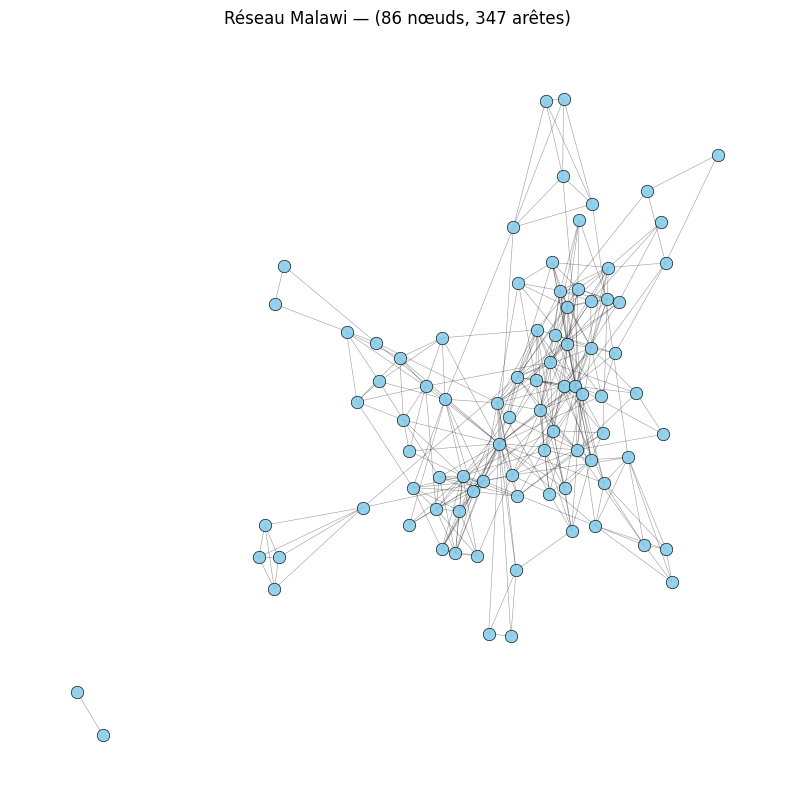
\includegraphics[width=0.90\linewidth]{images/article2/1.png}
\caption{Réseau de contacts du Malawi}
\end{figure}

Le réseau observé est presque entièrement connecté, ce qui suggère une communauté socialement soudée. 
Le \textbf{degré moyen} est de \textbf{8.07}, indiquant un niveau notable de connectivité, tandis que le \textbf{degré maximal} atteint 
\textbf{31}, révélant l’existence de personnes très actives socialement.

Le \textbf{coefficient de clustering}, égal à \textbf{0.5269}, constitue l’un des résultats les plus marquants. 
Il montre une densité exceptionnelle de triangles, traduisant des sous-groupes fortement cohésifs, sans doute liés 
aux ménages.

La \textbf{distance moyenne} de \textbf{2.6153} et le \textbf{diamètre} limité à \textbf{5} indiquent une structure compact. 
Le réseau présente ainsi les caractéristiques typiques d’un small-world : forte densité locale et communication rapide 
à l’échelle globale.

\section{Analyse des centralités}

\subsection{Betweenness Centrality}

La \textbf{betweenness centrality} met en évidence les individus jouant un rôle d’intermédiaire entre différentes parties 
du réseau. Le nœud \textbf{16} se distingue particulièrement avec une valeur de \textbf{0.3197}, nettement supérieure 
à celles des nœuds 81 et 74.  
Il occupe une position stratégique de pont entre différentes parties du réseau.

\subsection{Eigenvector Centrality}

La \textbf{eigenvector centrality} identifie les individus appartenant au cœur des structures les plus connectées. 
Les nœuds \textbf{70}, \textbf{54}, \textbf{15}, \textbf{63} et \textbf{48} obtiennent les valeurs les plus élevées 
(par exemple \textbf{0.5464} pour le nœud 70).  

Ils forment un noyau central où l’influence sociale est renforcée par la proximité avec d’autres individus centraux. 
Ces nœuds jouent un rôle d’ancrage dans la structure interne du village.

\subsection{PageRank}

Le \textbf{PageRank} met en évidence l’importance dynamique des individus. 
Le nœud \textbf{16} présente une valeur élevée de \textbf{0.02835}, suivi des nœuds \textbf{70} 
(\textbf{0.02410}) et \textbf{54} (\textbf{0.02026}).  

Ces mesures confirment l’existence de deux types d’acteurs clés : des intermédiaires structurants 
et un noyau dense d’individus influents.

\subsection{Closeness Centrality}

La \textbf{closeness centrality} renseigne sur la proximité moyenne d’un individu avec le reste du réseau. 
Le nœud \textbf{16} présente une valeur de \textbf{0.5845}, ce qui confirme sa position centrale. 
Les nœuds \textbf{81} (\textbf{0.5389}), \textbf{74} (\textbf{0.5061}) et \textbf{86} suivent avec des valeurs élevées.

La superposition d’une \textbf{betweenness} élevée et d’une \textbf{closeness} élevée confirme que le nœud 16 
joue simultanément le rôle d’intermédiaire et de centre géométrique du réseau.

\section{Comparaison avec des modèles aléatoires}

\subsection{Modèle \textit{Erdős–Rényi}}

Le modèle \textbf{Erdős–Rényi} permet de mesurer dans quelle mesure la structure observée pourrait émerger du hasard.  
Le \textbf{clustering moyen} des graphes ER atteint seulement \textbf{0.0976}, loin du clustering réel \textbf{0.5269}.  
La \textbf{variance des degrés} y est également beaucoup plus faible (\textbf{7.27} contre \textbf{26.13}).  

La \textbf{distance moyenne} observée dans les graphes ER est de \textbf{2.3389}, légère- ment inférieure à celle du réseau 
réel, ce qui reflète l’absence de structure interne.  

Enfin, la \textbf{modularity} obtenue dans ER est d’environ \textbf{0.292}, très éloignée de la valeur réelle \textbf{0.893}.  
Le réseau ne peut donc pas être assimilé à un graphe aléatoire simple.

\subsection{Configuration Model}

Le \textbf{Configuration Model}, qui conserve la distribution exacte des degrés, ne parvient pas davantage à reproduire 
les caractéristiques du réseau réel. Le \textbf{clustering} n’y atteint que \textbf{0.1393}, et la \textbf{modularity} seulement 
\textbf{0.3013}.  

Bien que la \textbf{distance moyenne} simulée (\textbf{2.4256}) soit proche de celle du réseau réel, ces modèles restent incapables 
de recréer l’intensité des communautés. Cela montre que la structure observée ne provient pas des degrés, 
mais d’une organisation sociale réelle et forte.

\section{Marche aléatoire}

La marche aléatoire, qui mesure la dynamique de visite des nœuds, met en évidence les individus les plus susceptibles 
d’être atteints lors d’un parcours au hasard. Le nœud \textbf{16} obtient une proportion de visites de \textbf{0.046}, 
suivi par les nœuds 81, 86, 74 et 70.  

Cela confirme que certaines personnes concentrent naturellement une part importante de la dynamique sociale, 
en raison de leur positionnement structurel.



L’analyse des contacts par heure met en évidence des variations significatives de l’activité sociale. 
Les heures \textbf{30} et \textbf{31} présentent des pics importants, avec respectivement \textbf{9217} et \textbf{9902} contacts.  

Ces fluctuations suggèrent l’existence de routines collectives ou de moments de rassemblement intense, montrant que 
le réseau n’est pas seulement structuré spatialement, mais également temporellement.



% =============================================================


% =============================================================


% =============================================================
\section{Analyse communautaire}
Comme l'algorithme de Louvain  a déjà été présenté dans l'article d'origine, nous nous concentrons ici sur deux autres approches complémentaires.   
\subsection{Méthodes basées sur des marches aléatoires}

Les méthodes fondées sur des marches aléatoires exploitent la manière dont un flux 
(d’information, d’individus) se déplace spontanément dans le réseau.
Elles sont particulièrement pertinentes pour analyser la cohésion interne des groupes
et la dynamique sociale du village.

Nous appliquons ici deux méthodes classiques : \textbf{Infomap} et \textbf{Walktrap}.

% ===============================================================
\subsubsection*{Infomap : partitionnement basé sur le flux d'information}

Infomap repose sur le \emph{Map Equation}, qui mesure la capacité à compresser
la description d’une marche aléatoire sur le réseau.  
Si une marche aléatoire tend à rester longtemps dans une même communauté,
alors la structure possède une organisation modulaire cohérente.

L’exécution d’Infomap sur le réseau Malawi donne :

\begin{itemize}
    \item \textbf{10 communautés détectées}, 
    \item tailles : $[37,\, 13,\, 8,\, 4,\, 6,\, 5,\, 5,\, 3,\, 3,\, 2]$.
\end{itemize}

Cette partition montre une structure où un grand module central (37 individus)
coexiste avec plusieurs petits ensembles fortement cohésifs.
Cela suggère que le village ne se compose pas uniquement de ménages isolés,
mais d’agrégats sociaux plus larges, où certains clusters regroupent plusieurs foyers.

% ===============================================================
\subsubsection*{Walktrap : communautés détectées via marches courtes}

Walktrap s’appuie sur l’idée que des marches aléatoires courtes restent
piégées dans les communautés. La méthode calcule des distances entre nœuds
en comparant leurs signatures de marche aléatoire.

L’application de Walktrap donne :

\begin{itemize}
    \item \textbf{11 communautés détectées}, 
    \item tailles : $[17,\, 3,\, 22,\, 3,\, 12,\, 6,\, 5,\, 8,\, 5,\, 3,\, 2]$.
\end{itemize}

Walktrap identifie des modules légèrement plus nombreux qu’Infomap,
avec notamment deux communautés moyennes (17 et 22 membres) et plusieurs
petits groupes correspondant à des ménages denses ou micro-communautés locales.

Cette structuration, basée sur la proximité dynamique entre individus,
reflète fidèlement l’organisation sociale du village :  
des foyers fortement cohésifs reliés entre eux par des liens plus faibles,
exactement comme décrit dans l’article original.

% ===============================================================
\subsubsection*{Comparaison des méthodes basées sur la marche aléatoire}

Infomap et Walktrap produisent des résultats cohérents mais complémentaires :

\begin{itemize}
    \item Infomap met en évidence un \textbf{macro-groupe dominant} de 37 individus,
          signe d’un flux social très concentré autour de certains clusters.
    \item Walktrap révèle une structure \textbf{méso-échelle} plus détaillée,
          avec 11 communautés dont plusieurs de taille moyenne (12 à 22 individus).
\end{itemize}

Ces deux méthodes contrastent avec Louvain pondéré, qui segmente davantage
le réseau (22 communautés), car Louvain exploite fortement les variations de poids.

Les méthodes basées sur la marche aléatoire montrent au contraire que,
d’un point de vue dynamique,  

\begin{itemize}
    \item les ménages ne sont pas des modules isolés,
    \item plusieurs d’entre eux fonctionnent comme des blocs sociaux plus larges,
    \item le village possède une structure communautaire hiérarchique,
          allant du ménage vers des communautés agrégées.
\end{itemize}

Ainsi, Infomap et Walktrap révèlent des caractéristiques sociales clés du réseau :
la coexistence d’un noyau central très interconnecté et d’une périphérie composée
de petits groupes familiaux.



% =============================================================
\section{Spectre du Laplacien et dynamique de consensus}

L’analyse spectrale constitue un outil fondamental pour comprendre la structure 
interne d’un réseau. Elle permet d’identifier les composantes connexes, 
de quantifier la cohésion des communautés et d’étudier la dynamique 
de propagation ou de synchronisation sur le graphe. Dans cette section, 
nous analysons le réseau Malawi à travers trois approches complémentaires :
le \textbf{spectral clustering}, le \textbf{spectre du Laplacien normalisé} 
et la \textbf{dynamique de consensus} $\dot{x}=-Lx$.

% =============================================================
\subsection{Spectral clustering}

Nous appliquons un spectral clustering en fixant le nombre de communautés à 
$k = 8 $, conformément au résultat obtenu avec Louvain non pondéré dans l’article de référence.

Le résultat obtenu est le suivant :

\[
\text{8 communautés avec tailles } 
[41,\ 21,\ 6,\ 5,\ 5,\ 3,\ 3,\ 2].
\]



Ces tailles montrent une structure modulaire cohérente 
quelques communautés de taille moyenne dominent la décomposition, 
accompagnées de plusieurs groupes plus petits, probablement liés 
à des ménages ou sous-ménages.

% =============================================================
\subsection{Valeurs propres du Laplacien normalisé}

Le calcul des dix plus petites valeurs propres du Laplacien normalisé donne :

\[
\lambda = 
\begin{bmatrix}
0.000000 \\
0.000000 \\
0.067425 \\
0.132788 \\
0.147327 \\
0.184823 \\
0.232372 \\
0.298524 \\
0.312749 \\
0.331314
\end{bmatrix}.
\]

Ces résultats permettent plusieurs observations majeures :

\begin{enumerate}
    \item \textbf{Présence de deux valeurs propres nulles.}  
Selon le théorème spectral du Laplacien, 
La présence de deux valeurs nulles indique donc que le réseau Malawi n’est pas entièrement connecté : il se compose d’une grande composante principale et d’une petite composante isolée.
Cette composante secondaire regroupe des individus n’ayant enregistré aucun contact avec le reste du village, probablement parce qu’ils ont été très peu présents ou ont porté le capteur de manière incorrecte durant la période d’observation.

    \item \textbf{Valeurs propres faibles ($\lambda_2$, $\lambda_3$, …).}  
    Les valeurs proches de zéro ($0.067$, $0.133$, $0.147$) indiquent 
    une séparation nette entre les ménages.  
    Cela révèle une structure modulaire très forte : densité interne élevée dans les communautés,
    faible connectivité entre communautés.
        
    En comparaison, l’article du Malawi rapporte également une forte modularité et une structure 
    fortement contrainte par les ménages.  
    L’analyse spectrale confirme rigoureusement ces observations.
\end{enumerate}

% =============================================================
\subsection{Dynamique de consensus}

Nous simulons la dynamique continue :
\[
\dot{x} = -Lx,
\]
où chaque nœud possède un état initial aléatoire.  
Cette dynamique modélise la convergence d’opinions, d’informations ou de comportements.

\begin{figure}[H]
\centering
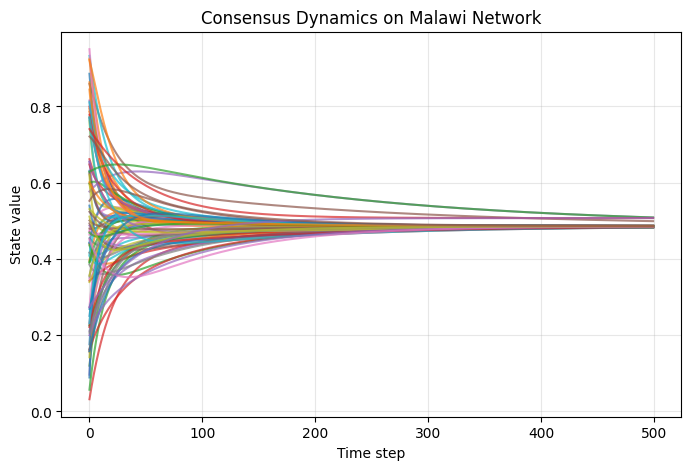
\includegraphics[width=0.85\linewidth]{images/article2/3.png}
\caption{Dynamique de consensus sur le réseau Malawi.}
\end{figure}

L’interprétation est la suivante :

\begin{itemize}
    \item Les courbes convergent rapidement à l’intérieur d’un ménage,  
    ce qui reflète une \textbf{forte cohésion locale}.
    \item La convergence globale est beaucoup plus lente :  
    cela correspond au fait que les liens inter-ménages sont faibles.
    \item Le plateau final correspond à un consensus global stable.
\end{itemize}

Ce phénomène illustre la \textbf{séparation d’échelles} décrite au Chapitre~6 :
les clusters internes se stabilisent très vite, tandis que 
l’harmonisation entre clusters est graduelle.


\section{Structure core--periphery}

\subsection{k-core decomposition}

Dans le cas du réseau Malawi, le graphe complet comporte deux composantes connexes.
Or, la décomposition en $k$-cores n’est pleinement interprétable que sur un graphe connexe.  
Pour cette raison, nous appliquons l’analyse exclusivement sur la 
\textbf{plus grande composante connexe (LCC)}, qui contient l’essentiel des interactions
sociales du village.

\medskip

La décomposition en $k$-cores permet d’identifier la structure interne du réseau.
Un $k$-core est un sous-graphe maximal dans lequel chaque nœud possède un degré au 
moins égal à $k$.

\medskip
L’analyse effectuée sur la LCC du réseau Malawi donne les résultats suivants :

\begin{itemize}
    \item \textbf{$k$-core maximal : 7} ;
    \item \textbf{taille du noyau (7-core) : 31 individus} ;
\end{itemize}

\medskip

Ces résultats révèlent une structure interne fortement hiérarchisée.  
Le noyau ($7$-core) regroupe les individus les plus connectés du village, 
probablement des adultes actifs ou des Health Surveillance Assistants (HSA),
dont le rôle social central a été souligné dans l’article scientifique.  



\begin{figure}[H]
\centering
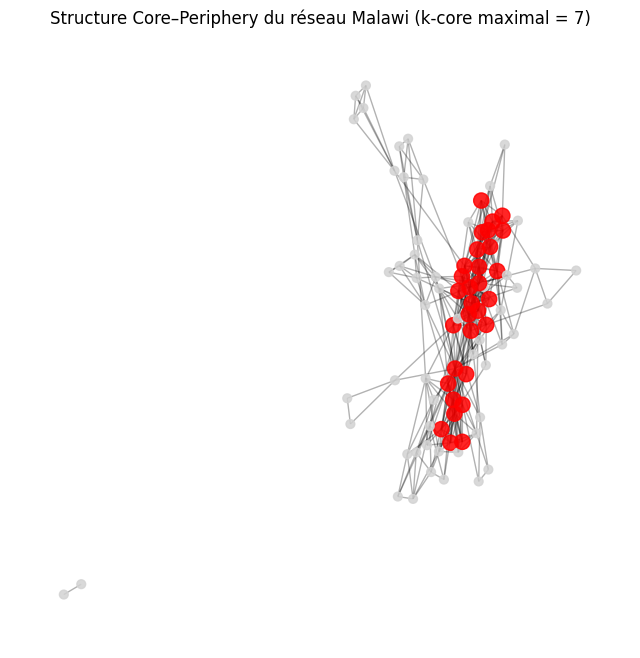
\includegraphics[width=0.75\linewidth]{images/article2/6.png}
\caption{Structure k-core du réseau Malawi (analyse sur la LCC, $k$-core maximal = 7).}
\label{fig:kcore}
\end{figure}

Cette organisation met en évidence un \textbf{noyau social dense }.
Cela confirme que le réseau Malawi est caractérisé par une forte cohésion interne, 
structurée autour d’un groupe central jouant un rôle crucial dans la connectivité globale
et dans la propagation potentielle d’information ou d’infections.


\subsection{Structure core--periphery basée sur les marches aléatoires}

En complément de la décomposition en $k$-cores, qui repose uniquement sur le degré des nœuds,
nous appliquons une méthode alternative de détection de la structure
core--periphery fondée sur les marches aléatoires, telle que présentée au
Chapitre~8 du syllabus.

\medskip

Cette approche repose sur une interprétation dynamique de la centralité.
L’idée principale est d’analyser le comportement d’un marcheur aléatoire sur le réseau :
un ensemble de nœuds est considéré comme central s’il est difficile pour une marche
aléatoire de le quitter.

\medskip

Soit $S$ un ensemble de nœuds. La \emph{probabilité de persistance} $\alpha_S$ est définie comme
la probabilité qu’un marcheur aléatoire, conditionné à être dans $S$ à un instant donné,
reste dans $S$ au pas de temps suivant. Dans le cas d’un graphe non orienté, cette quantité
s’écrit :
\[
\alpha_S = \frac{\sum_{i,j \in S} A_{ij}}{\sum_{i \in S} k_i},
\]
où $A_{ij}$ est la matrice d’adjacence et $k_i$ le degré du nœud $i$.

\medskip

Afin d’identifier la structure core--periphery, nous utilisons un algorithme glouton.
L’algorithme démarre à partir d’un nœud de degré minimal, puis ajoute itérativement
le nœud qui minimise la valeur de $\alpha_S$.
À chaque étape, la valeur de $\alpha_S$ associée à l’ajout d’un nœud définit sa
\emph{coreness} $\alpha_i$.
Plus $\alpha_i$ est élevé, plus le nœud est central du point de vue de la dynamique
de marche aléatoire.

\medskip

Plutôt que de fixer un seuil unique, nous considérons $\alpha$ comme un paramètre continu.
Pour chaque valeur de $\alpha \in [0,1]$, nous définissons la
\emph{$\alpha$-périphérie} comme l’ensemble des nœuds satisfaisant $\alpha_i \le \alpha$.
Cette approche permet d’observer la dynamique d’absorption progressive des nœuds
depuis la périphérie vers le cœur.

\medskip

L’analyse réalisée sur la plus grande composante connexe (LCC), qui contient 84 nœuds,
montre une augmentation progressive et régulière de la taille de la périphérie lorsque
$\alpha$ augmente. Pour $\alpha = 0.1$, la périphérie contient 28 nœuds, tandis que
le cœur regroupe les 56 nœuds restants.

\medskip

\begin{figure}[H]
\centering
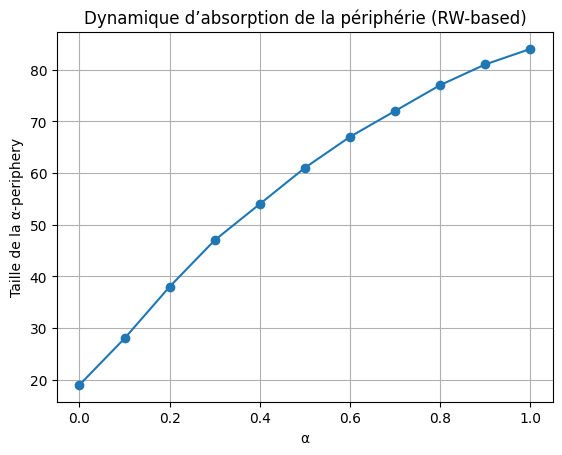
\includegraphics[width=0.75\linewidth]{images/article2/7.png}
\caption{Dynamique d’absorption de la périphérie en fonction de $\alpha$ sur le réseau Malawi.}
\label{fig:rw_dynamics}
\end{figure}

\medskip

Contrairement à la décomposition en $k$-cores, la structure obtenue par la méthode
RW-based ne repose pas uniquement sur le degré des nœuds, mais sur leur rôle global
dans la stabilité des trajectoires de marche aléatoire.
Le cœur RW-based est ainsi plus large que le $k$-core maximal, ce qui suggère que
la centralité dynamique dépasse la simple connectivité locale.

\medskip

Cette analyse met en évidence le caractère complémentaire des deux approches :
le $k$-core identifie les nœuds fortement connectés localement, tandis que la méthode
RW-based capture une notion plus globale et dynamique de centralité au sein du réseau.







% =============================================================
\section{Dynamique épidémique}

L’étude de la diffusion d’une infection dans le réseau Malawi s’appuie sur les
outils vus au Chapitre~9 : valeur propre dominante, identification des
\textit{superspreaders} et simulation du modèle SIR.  
Toutes les analyses sont effectuées sur la \textbf{composante géante} du réseau,
qui contient ici \textbf{84 nœuds}.

% =============================================================
\subsection{Seuil épidémique}

Le seuil fondamental d’invasion d’une épidémie dans un réseau est donné par :
\[
\frac{\beta}{\mu} > \frac{1}{\lambda_{\max}},
\]
où $\lambda_{\max}$ est la plus grande valeur propre de la matrice d’adjacence.

Le calcul donne :
\[
\lambda_{\max} = 11.9348,
\qquad
\frac{1}{\lambda_{\max}} = 0.0838.
\]

Ainsi, une maladie se propage dans la population si son ratio
de contagiosité $\beta/\mu$ dépasse \textbf{0.0838}.  
Ce résultat signifie qu’une infection même modérément transmissible
peut envahir rapidement le village, ce qui confirme la forte connectivité
structurelle observée dans les étapes précédentes.

% =============================================================
\subsection{Identification des superspreaders}

Les superspreaders sont identifiés via trois mesures de centralité définies
sur la composante géante : centralité de degré, eigenvector centrality
et distribution stationnaire de la marche aléatoire.

Les nœuds ayant les plus fortes valeurs dans ces mesures jouent un rôle
d’amplificateur potentiel dans la diffusion épidémique.

Le classement obtenu est le suivant  :

\[
\begin{array}{c|c|c|c}
\textbf{Node} & \textbf{Degree} & \textbf{Eigenvector} & \textbf{Stationary prob.} \\
\hline
16 & 31 & 0.257 & 0.0448 \\
81 & 26 & 0.311 & 0.0376 \\
69 & 18 & 0.144 & 0.0260 \\
74 & 17 & 0.234 & 0.0246 \\
70 & 16 & 0.224 & 0.0231 \\
\end{array}
\]

Le nœud \textbf{16} apparaît comme le super-propagateur principal, cumulant
haut degré, forte eigenvector centrality et probabilité stationnaire élevée.
Ce résultat est cohérent avec les analyses structurales et avec l’article qui
mentionne que certains adultes très actifs jouent un rôle disproportionné
dans les interactions sociales.


% =============================================================
\subsection{Simulation SIR}

Nous simulons la propagation d’une infection selon le modèle SIR avec :
\[
\beta = 0.03, \qquad \mu = 0.02.
\]

Deux scénarios opposés sont testés :

\begin{itemize}
    \item \textbf{Patient zéro = superspreader} (nœud 16) ;
    \item \textbf{Patient zéro = individu périphérique}.
\end{itemize}

\begin{figure}[H]
\centering
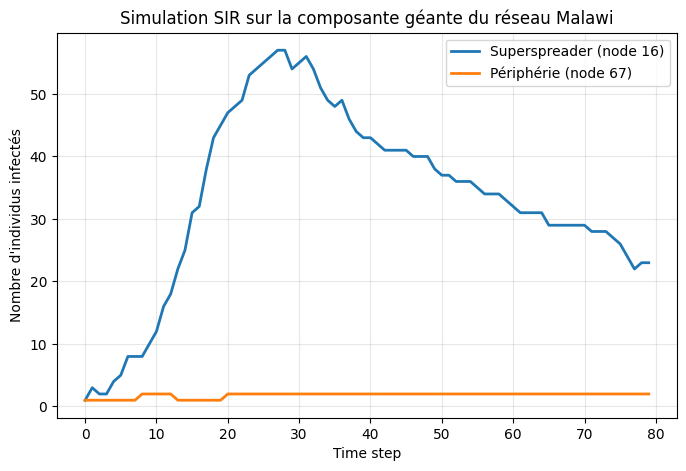
\includegraphics[width=0.80\linewidth]{images/article2/5.png}
\caption{Simulation SIR sur la composante géante du réseau Malawi.}
\end{figure}

Les résultats montrent une différence radicale :

\begin{itemize}
    \item Lorsqu’un \textbf{superspreader} est infecté, l’épidémie devient rapidement massive,
          dépassant plus de \textbf{50 individus infectés simultanément}.
    \item Lorsqu’un \textbf{nœud périphérique} est infecté, la propagation
          reste très limitée et s’éteint rapidement.
\end{itemize}

% =============================================================

\section{Interprétation générale} 

Ce travail a permis d’analyser la structure et les dynamiques du réseau de contacts
du village de Mdoliro (Malawi)en mobilisant les principaux outils du cours de \textit{Graph Mining}.

Les analyses montrent que le réseau est fortement structuré autour de
\textbf{ménages très cohésifs}, comme l’indiquent le clustering élevé, la modularité
exceptionnelle et la convergence rapide observée dans la dynamique de consensus
à l’échelle locale. Ces résultats confirment les conclusions de l’article scientifique
de référence.

Au-delà de cette organisation locale, l’étude met en évidence l’existence d’un
\textbf{noyau restreint d’individus centraux} jouant un rôle clé dans la connectivité
globale du réseau. Les mesures de centralité, les méthodes de détection de communautés
(\textit{Infomap} et \textit{Walktrap}), la décomposition en $k$-cores et l’analyse
core--periphery basée sur les marches aléatoires identifient de manière cohérente
ces acteurs, qui assurent la liaison entre les ménages.

La comparaison avec des modèles aléatoires montre que cette structure ne peut être
expliquée ni par le hasard ni par la seule distribution des degrés, mais reflète une
organisation sociale réelle et hiérarchique.

Enfin, l’analyse épidémique souligne les implications pratiques de cette structure :
la présence d’individus centraux rend le réseau vulnérable à une propagation rapide
des infections, comme l’illustrent les simulations SIR.

En conclusion, cette étude confirme et enrichit les résultats de l’article original
en proposant une analyse à la fois structurelle et dynamique du réseau Malawi.

% ---- (TOUT LE CONTENU MALAWI RESTE IDENTIQUE) ----
% Tu peux coller ici SANS MODIFICATION tout le reste

% ============================================================
% ============================================================

\section*{II- Réseau de contacts hospitalier}
\addcontentsline{toc}{section}{Étude de cas 2 — Réseau de contacts hospitalier}

\section{Introduction}

avec des valeurs atteignant \textbf{58} et \textbf{57} voisins (IDs 1193, 1164, 1115),
suivis par certains médecins \textbf{MED} (jusqu’à \textbf{53}).
Ces individus correspondent aux principaux hubs du réseau,
en interaction avec un grand nombre d’acteurs distincts.

\subsection{Strength}

Le cumul des durées de contacts est largement dominé par les \textbf{NUR}.
Les valeurs de strength les plus élevées dépassent \textbf{4000}
(ID 1115 : \textbf{4286}, ID 1210 : \textbf{4077}),
confirmant que les infirmiers concentrent les interactions les plus longues
et les plus fréquentes.

\subsection{Betweenness centrality}

Les valeurs de betweenness les plus importantes concernent principalement
des \textbf{NUR} (jusqu’à \textbf{0.0708} pour l’ID 1210),
ainsi que quelques \textbf{ADM} et \textbf{MED}.
Ces individus jouent un rôle d’intermédiaire entre différentes parties du réseau.

\subsection{Closeness centrality}

Les scores de closeness les plus élevés sont également observés
chez les \textbf{NUR}, avec des valeurs supérieures à \textbf{0.40}
(ID 1210 : \textbf{0.4088}),
ce qui reflète leur position centrale et leur proximité moyenne
au reste du réseau.

\subsection{Eigenvector centrality}

L’eigenvector centrality met en évidence un noyau fortement interconnecté
dominé par les \textbf{NUR}.
Les valeurs maximales atteignent \textbf{0.49} (IDs 1115 et 1210),
indiquant une forte connexion à d’autres nœuds eux-mêmes centraux.

\subsection{PageRank}

Le PageRank pondéré par la durée des contacts confirme ces observations.
Les scores les plus élevés sont obtenus par des \textbf{NUR},
avec des valeurs allant jusqu’à \textbf{0.0558} (ID 1115),
recouvrant largement les individus identifiés par le strength.

\subsection{Interprétation des centralités}

L’ensemble des mesures converge vers le même constat :
les \textbf{NUR}, puis les \textbf{MED}, occupent les positions les plus centrales
du réseau, à la fois en nombre de contacts, en durée cumulée
et en importance structurelle globale.
À l’inverse, les \textbf{PAT} et \textbf{ADM} apparaissent plus souvent
en périphérie, avec des niveaux de connectivité et d’influence plus faibles.


% ============================================================
\section{Comparaison avec des graphes modèles (null models)}
% ============================================================

L’objectif ici est de déterminer si les propriétés observées sont explicables par  le hasard pur (Erd\H{o}s--R\'enyi) ou par la seule distribution des degrés (Configuration Model).

\subsection{Erd\H{o}s--R\'enyi : hétérogénéité et hubs}

Le modèle ER $G(N,q)$ produit une distribution de degrés proche d’une loi de Poisson (concentrée autour du degré moyen).  
Or, le réseau réel est beaucoup plus \textbf{hétérogène} : il présente une queue plus lourde et des hubs marqués.

\begin{figure}[H]
\centering
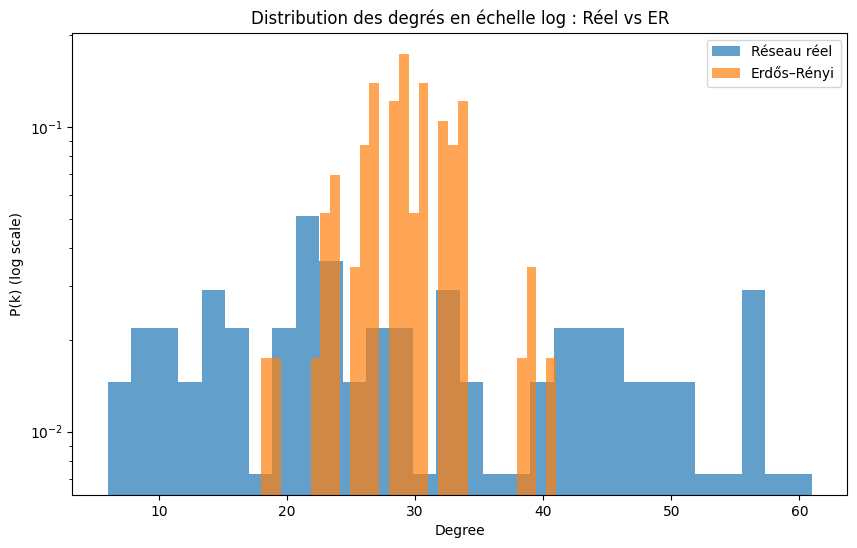
\includegraphics[width=0.90\linewidth]{images/article1/image1.png}
\caption{Distribution des degrés : réseau réel vs Erd\H{o}s--R\'enyi.}
\end{figure}

Conclusion : un graphe aléatoire simple ne peut pas reproduire l’organisation hospitalière.

\subsection{Configuration Model : triangles et organisation par rôle}

Le Configuration Model conserve la séquence de degrés, mais randomise les connexions.  
On observe alors des écarts structuraux importants :

\begin{itemize}
    \item \textbf{Clustering} : le réseau réel présente un clustering nettement plus élevé ($\approx 0.64$) que le CM ($\approx 0.40$), indiquant une forte présence de triangles liés aux équipes et aux soins répétés.
    \item \textbf{Distance moyenne} : légèrement plus faible dans le réseau réel ($1.59$ contre $1.70$), suggérant une connectivité renforcée via quelques individus centraux.
    \item \textbf{Assortativité par rôle} : négative dans le réseau réel ($r=-0.12$) et quasi nulle dans le CM, montrant que les interactions NUR--PAT et MED--PAT reflètent des contraintes fonctionnelles plutôt que la seule distribution des degrés.
\end{itemize}


\subsection{Interpretation des  modèles}

Le contrôle de la distribution des degrés ne suffit pas à reproduire la structure observée.
Le réseau réel reste caractérisé par une forte densité locale, des interactions dépendantes des rôles et une organisation non aléatoire liée au fonctionnement hospitalier.

% ============================================================
\section{Profil temporel des interactions}
% ============================================================

Les réseaux de contacts hospitaliers sont typiquement \textbf{rythmiques} : alternance jour/nuit, pics liés aux soins et aux transmissions.

\subsection{Nombre total de contacts par heure}

\begin{figure}[H]
\centering
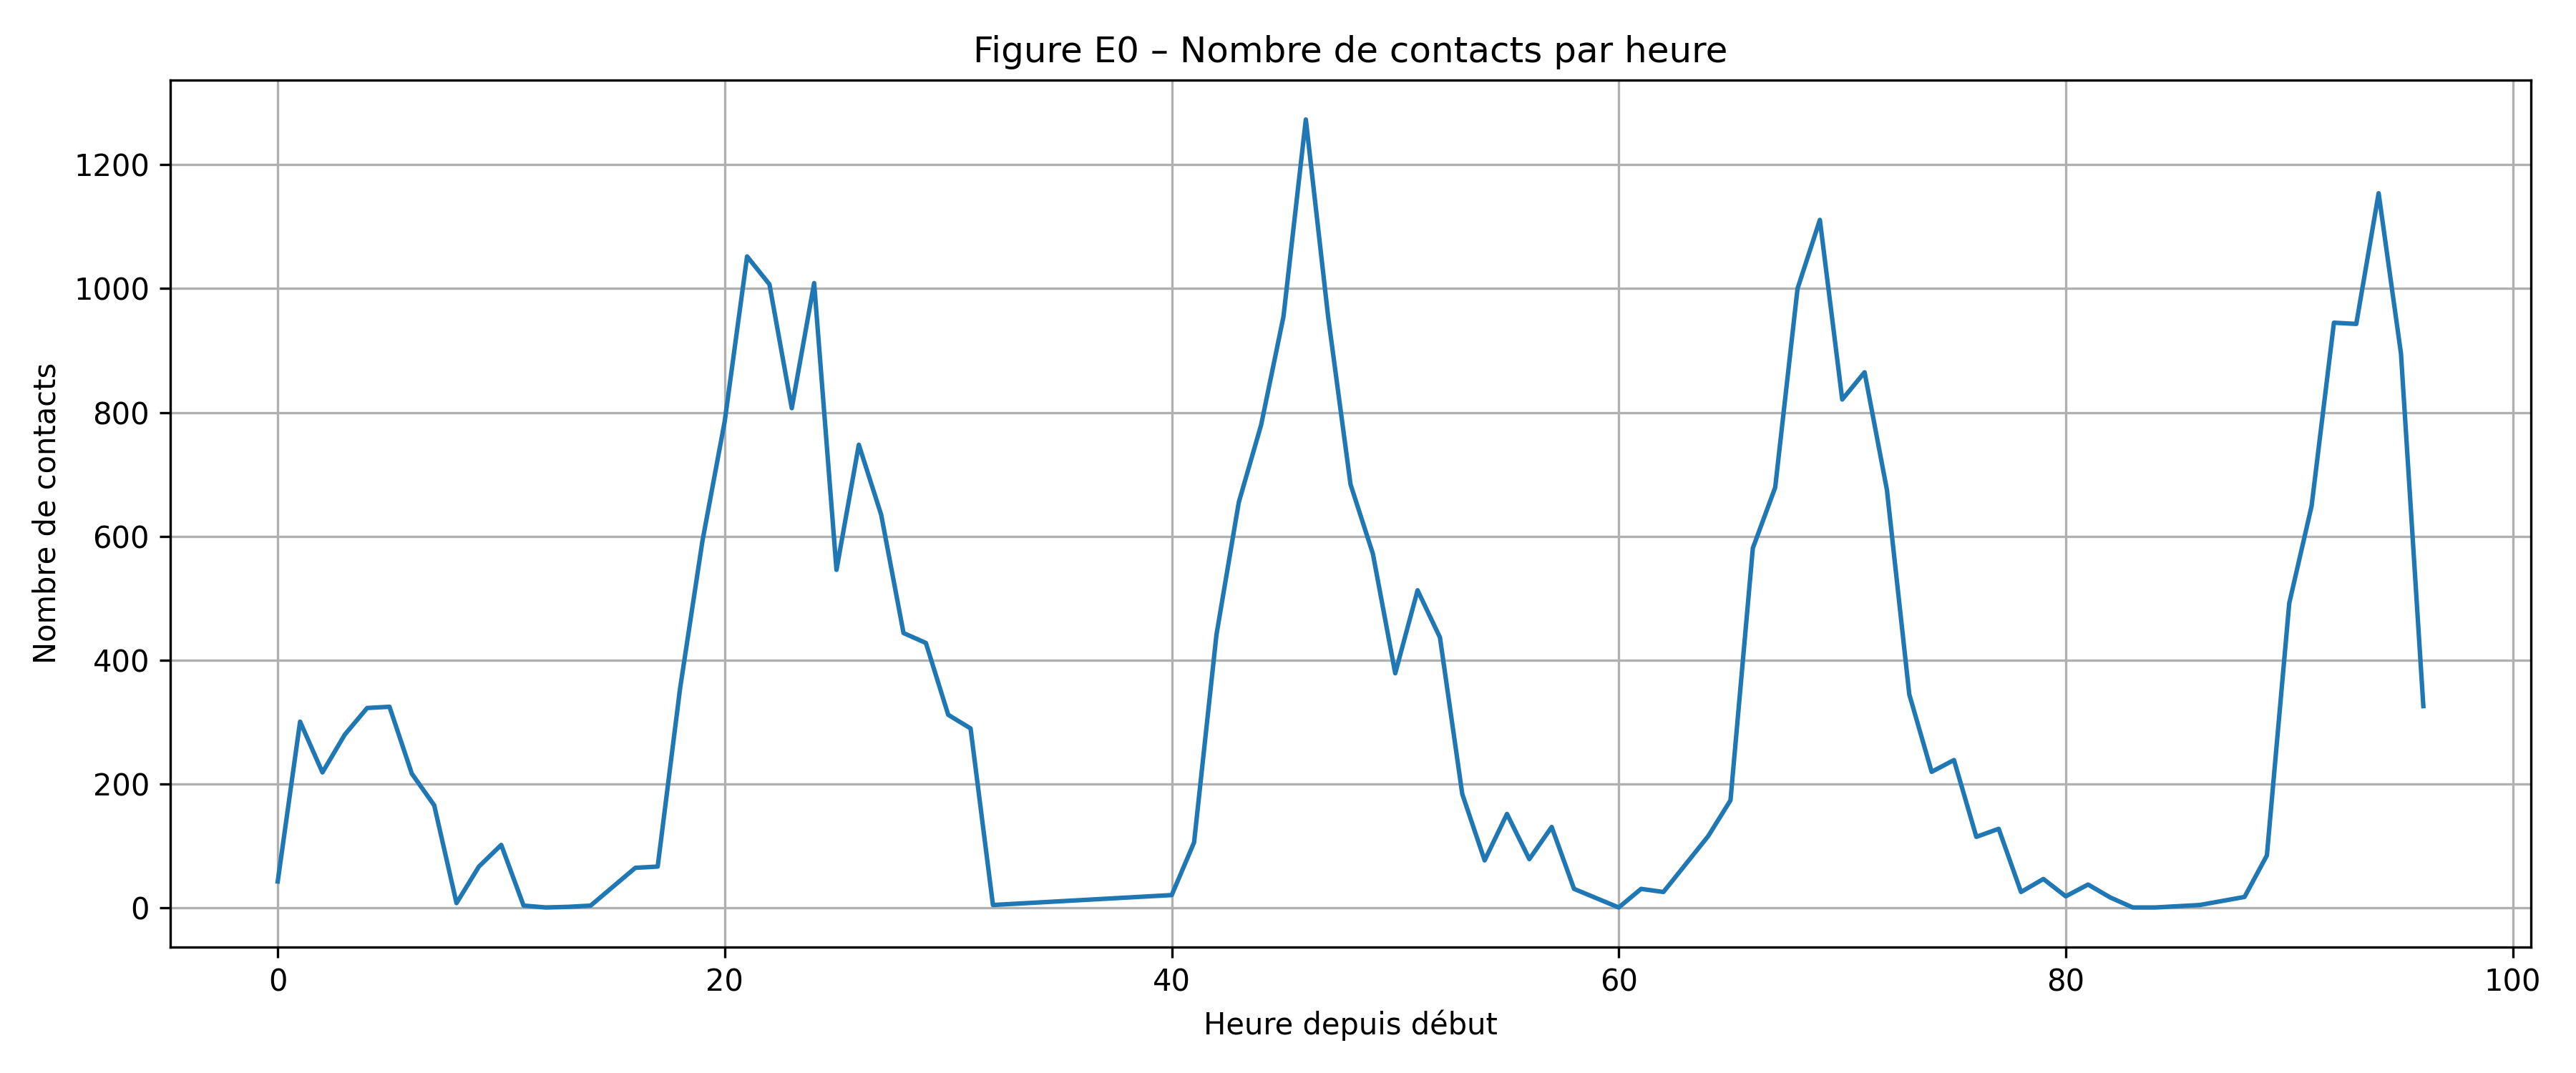
\includegraphics[width=0.90\linewidth]{images/article1/Figure_E0_contacts_par_heure.png}
\caption{Nombre total de contacts par heure.}
\end{figure}

On observe une structure \textbf{cyclique} :
pics marqués en journée (activité soignante) et creux nocturnes.  
Cela indique une organisation temporelle stable et répétitive.

\subsection{Contacts par type d’interaction}

\begin{figure}[H]
\centering
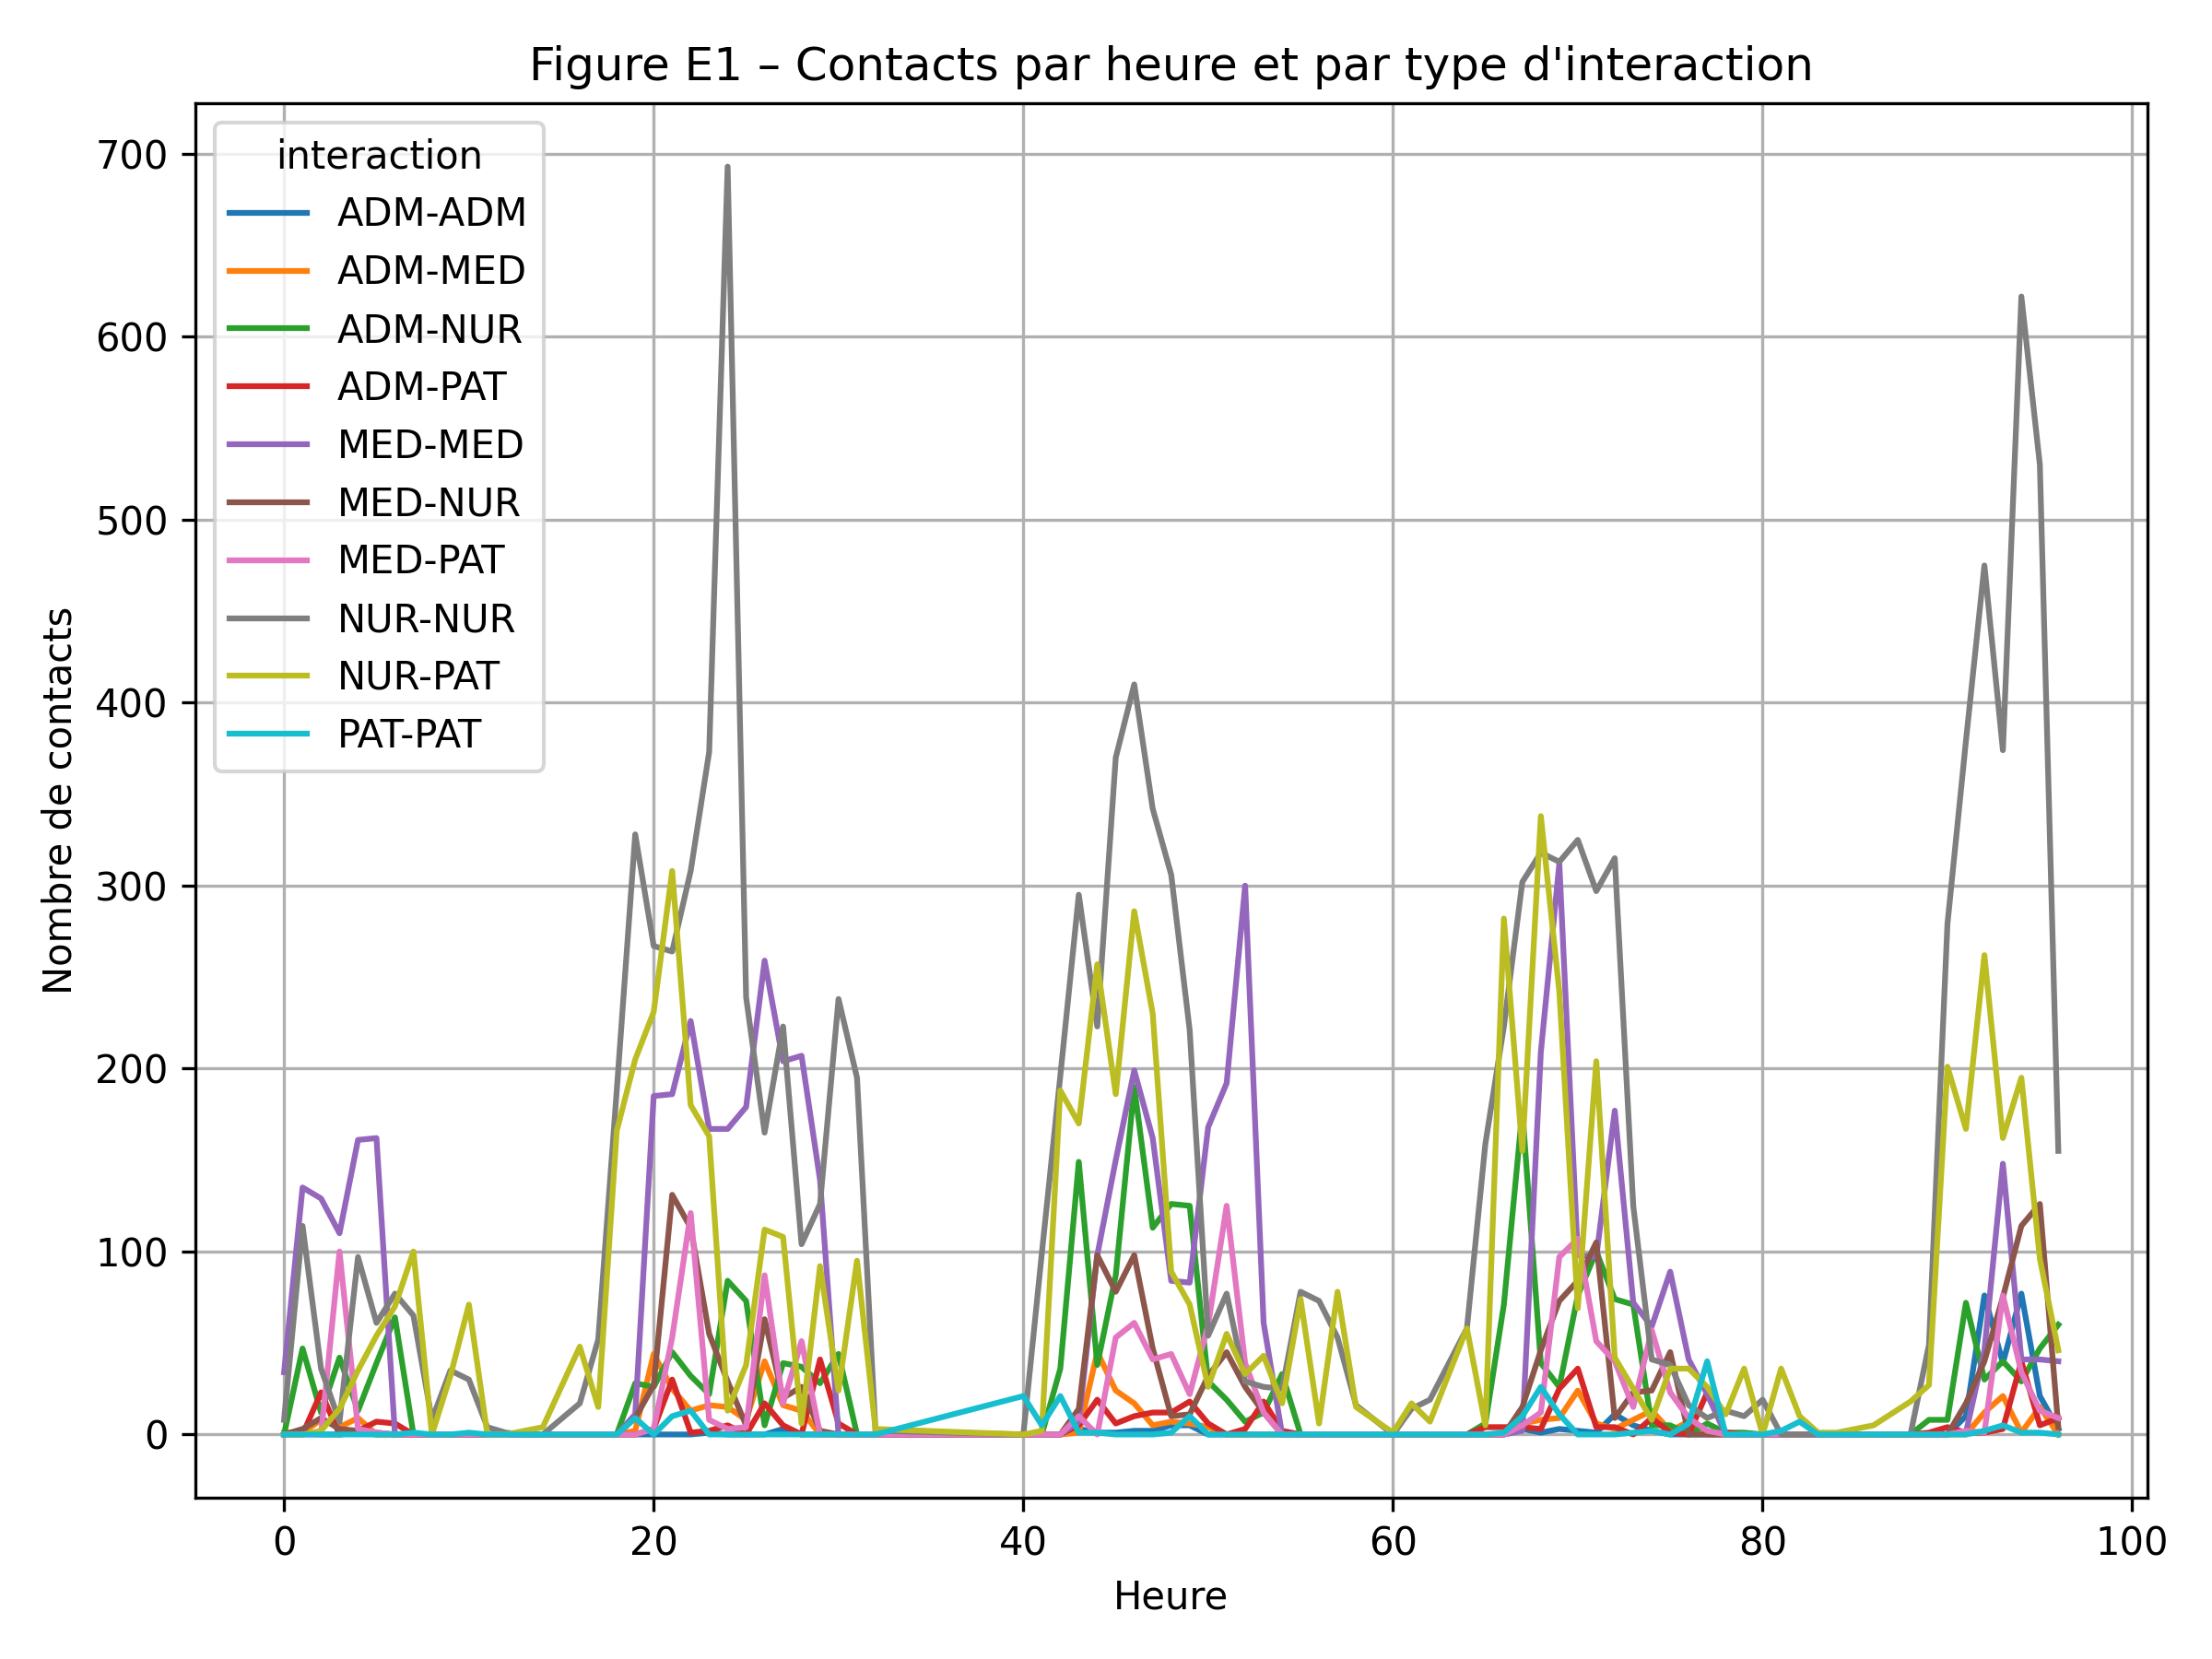
\includegraphics[width=0.90\linewidth]{images/article1/Figure_E1_contacts_par_role.png}
\caption{Contacts par heure selon le type d’interaction.}
\end{figure}

Les interactions \textbf{NUR--PAT} et \textbf{NUR--NUR} dominent :
les infirmiers sont l’interface opérationnelle entre patients et système hospitalier.  
Les \textbf{ADM} restent faibles et davantage internes à leur catégorie.

% ============================================================
\section{Stabilité du voisinage : similarité de Jaccard}
% ============================================================

\subsection{Définition}

Pour un individu $i$, si $N_1(i)$ est l’ensemble de ses voisins au jour 1 et $N_2(i)$ au jour 2 :
\[
J(i)=\frac{|N_1(i)\cap N_2(i)|}{|N_1(i)\cup N_2(i)|}.
\]


\subsection{Résultats par rôle}

\begin{figure}[H]
\centering
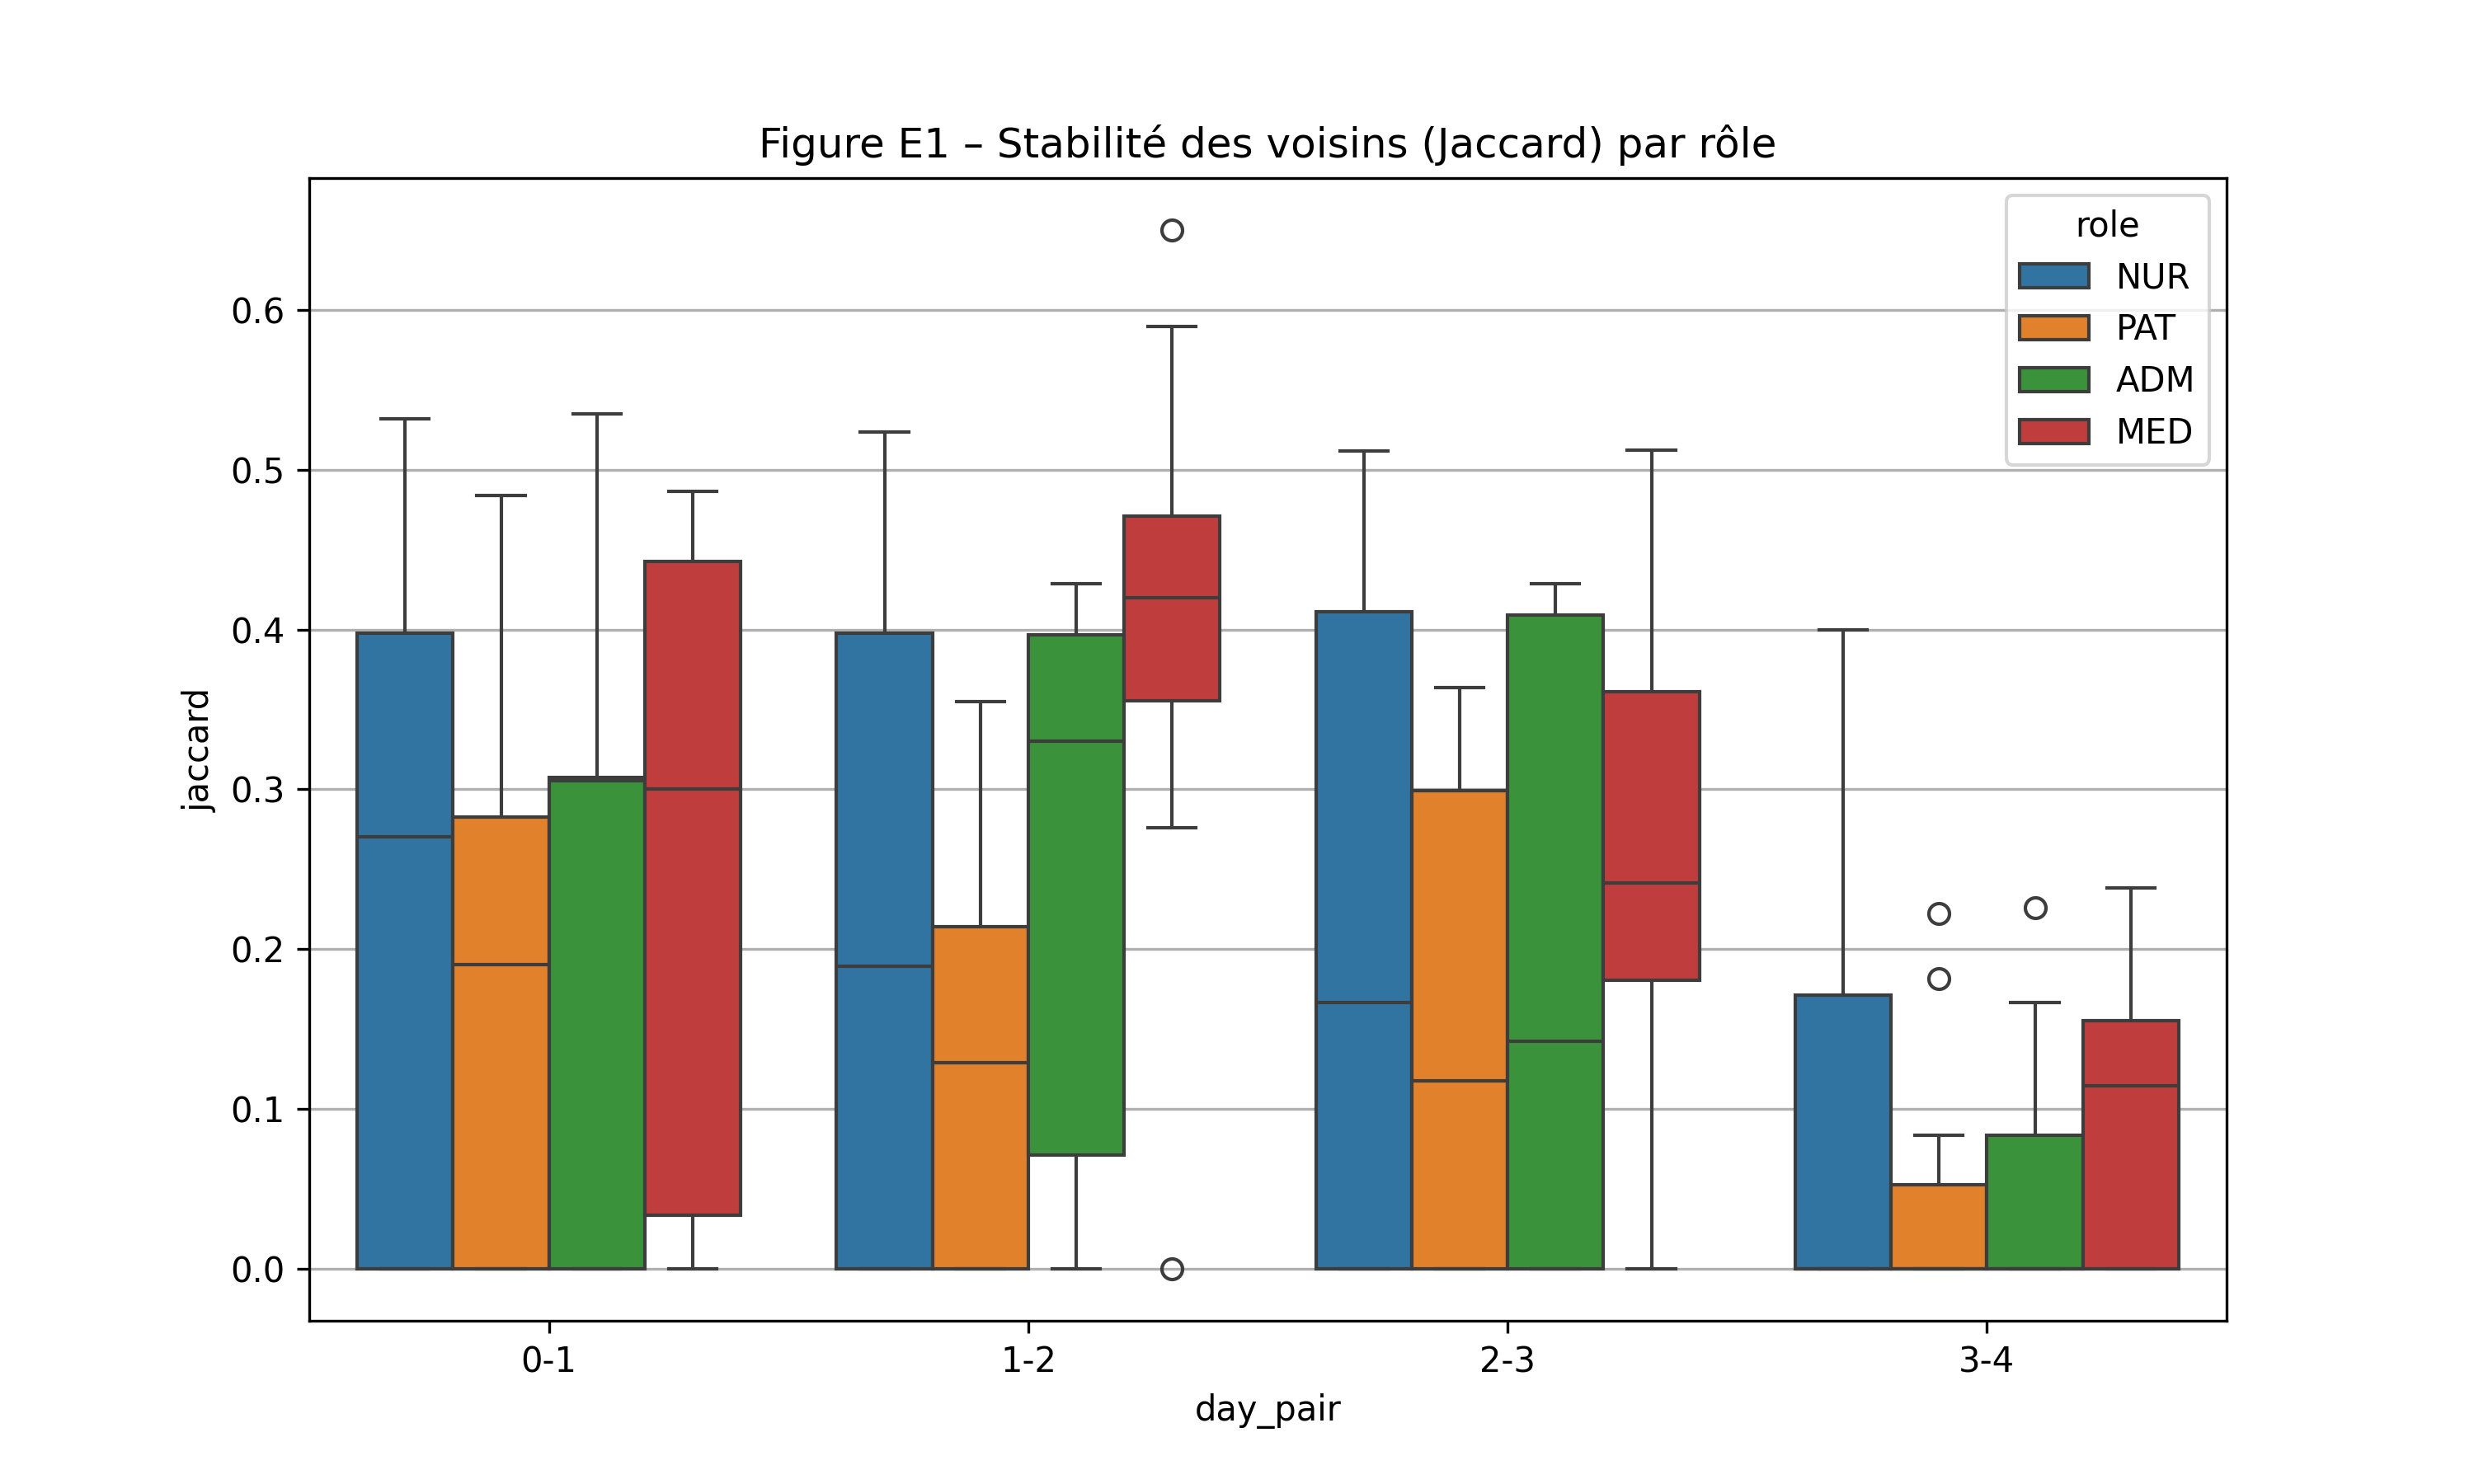
\includegraphics[width=0.85\linewidth]{images/article1/Figure_E1_stabilite_voisinage.png}
\caption{Stabilité des voisinages (Jaccard) par rôle.}
\end{figure}

\begin{itemize}
    \item \textbf{NUR} : stabilité élevée $\Rightarrow$ équipes et routines de soins.
    \item \textbf{MED} : stabilité intermédiaire.
    \item \textbf{PAT} : stabilité faible $\Rightarrow$ interactions dépendantes des soins, déplacements, état clinique.
\end{itemize}

Ainsi, le personnel présente une structure sociale stable, tandis que la partie patient est plus dynamique.

% ============================================================
\section{Structure temporelle : compacité et connectivité}
% ============================================================

On étudie ici comment la structure instantanée (par heure) évolue en termes de distances et connectivité globale.

\subsection{Diamètre}

\begin{figure}[H]
\centering
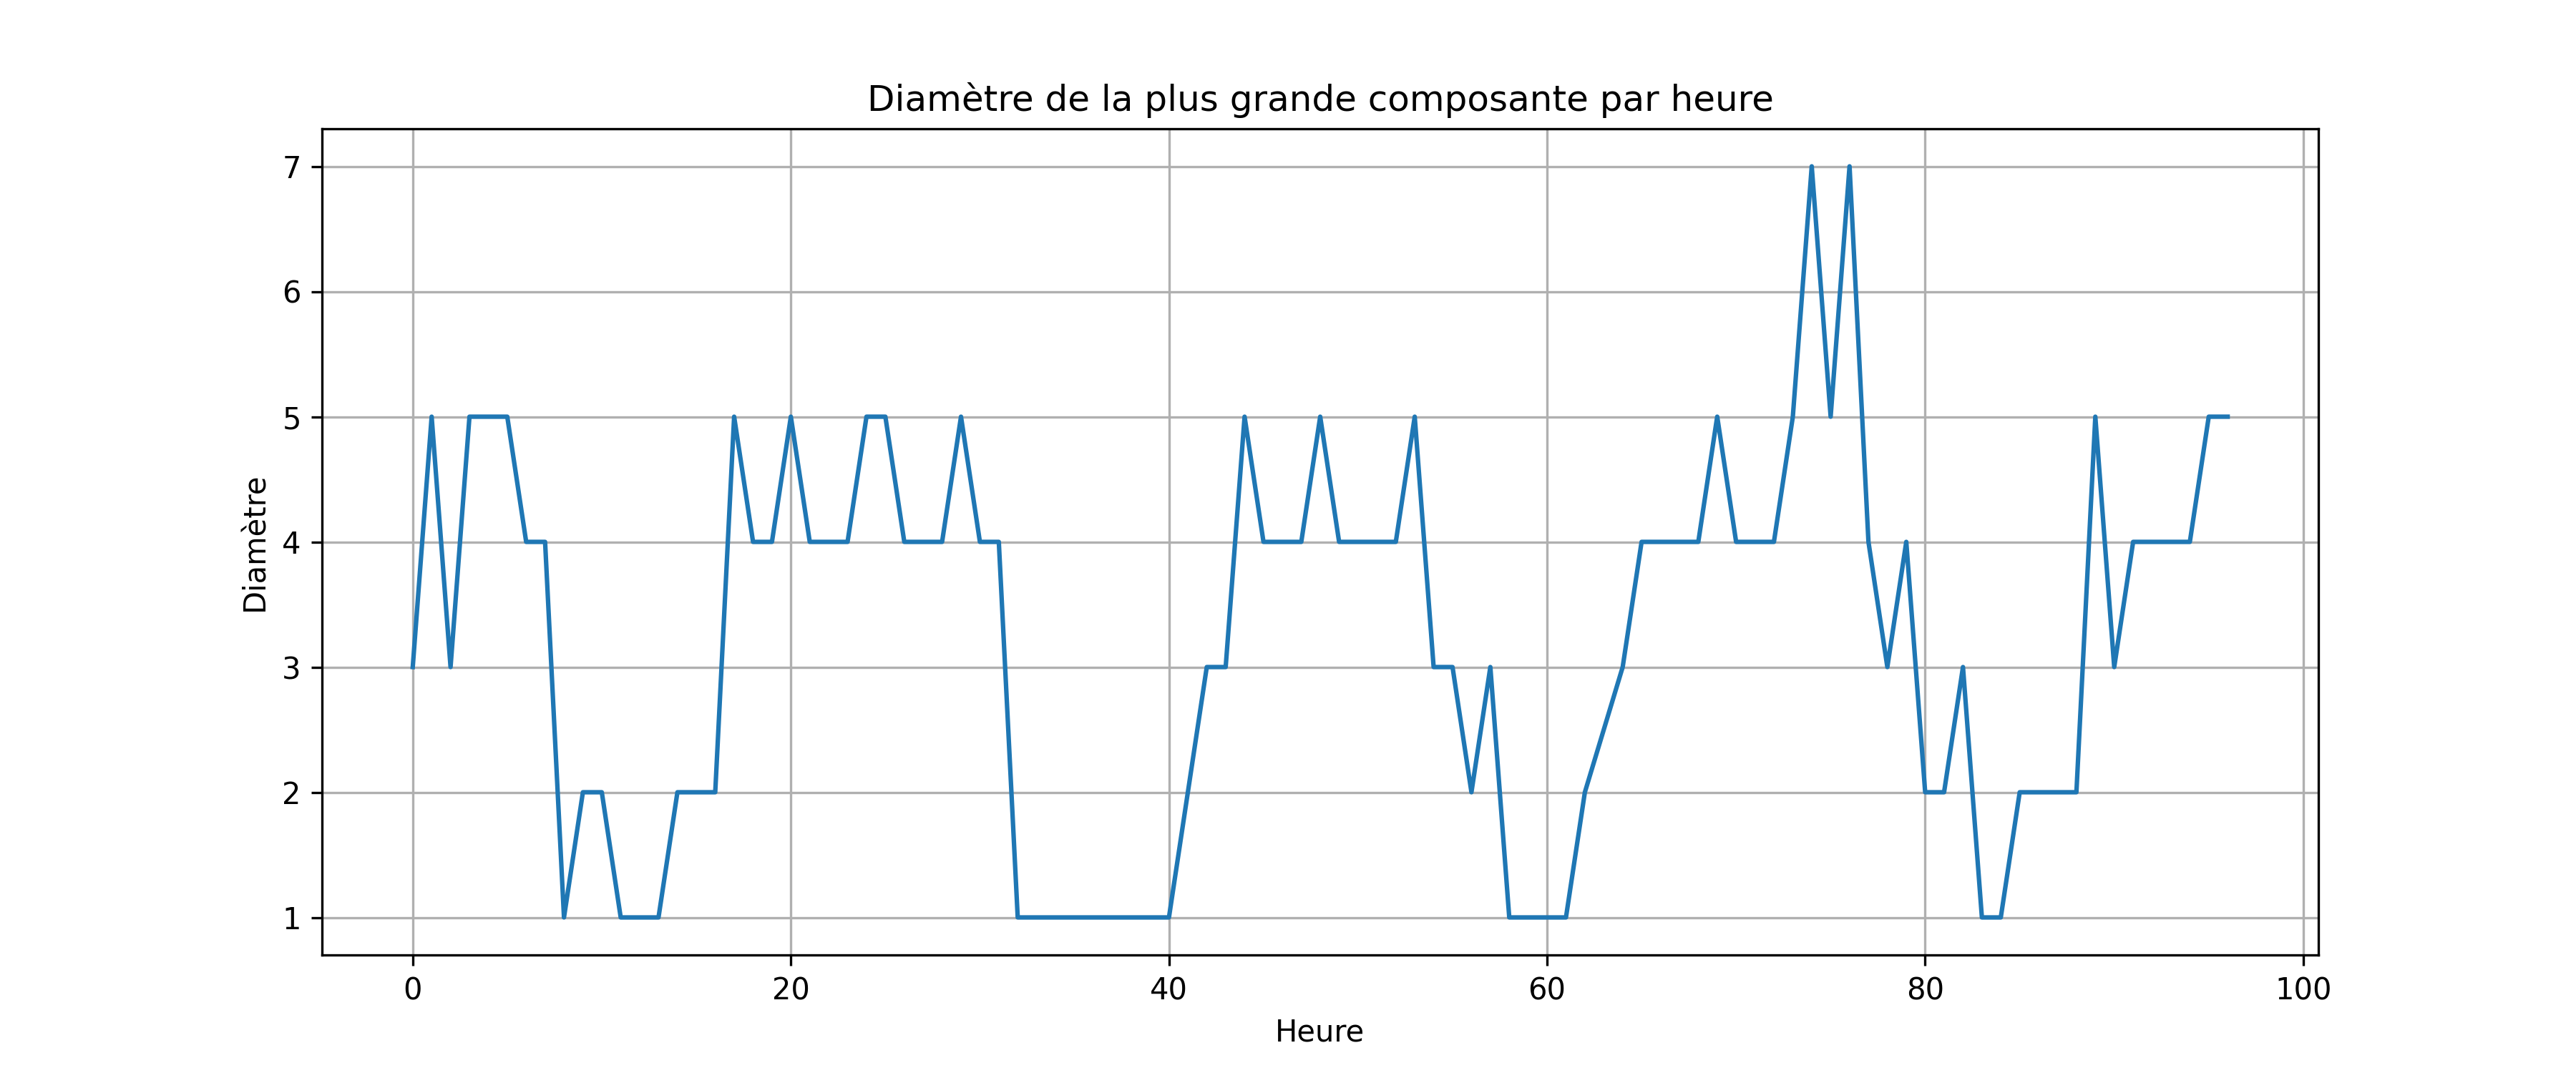
\includegraphics[width=0.90\linewidth]{images/article1/Figure_E2_diametre.png}
\caption{Diamètre de la plus grande composante.}
\end{figure}

Un diamètre entre 3 et 7 indique un réseau \textbf{compact} :
même dans les périodes moins actives, les distances restent faibles.

\subsection{Distance moyenne}

\begin{figure}[H]
\centering
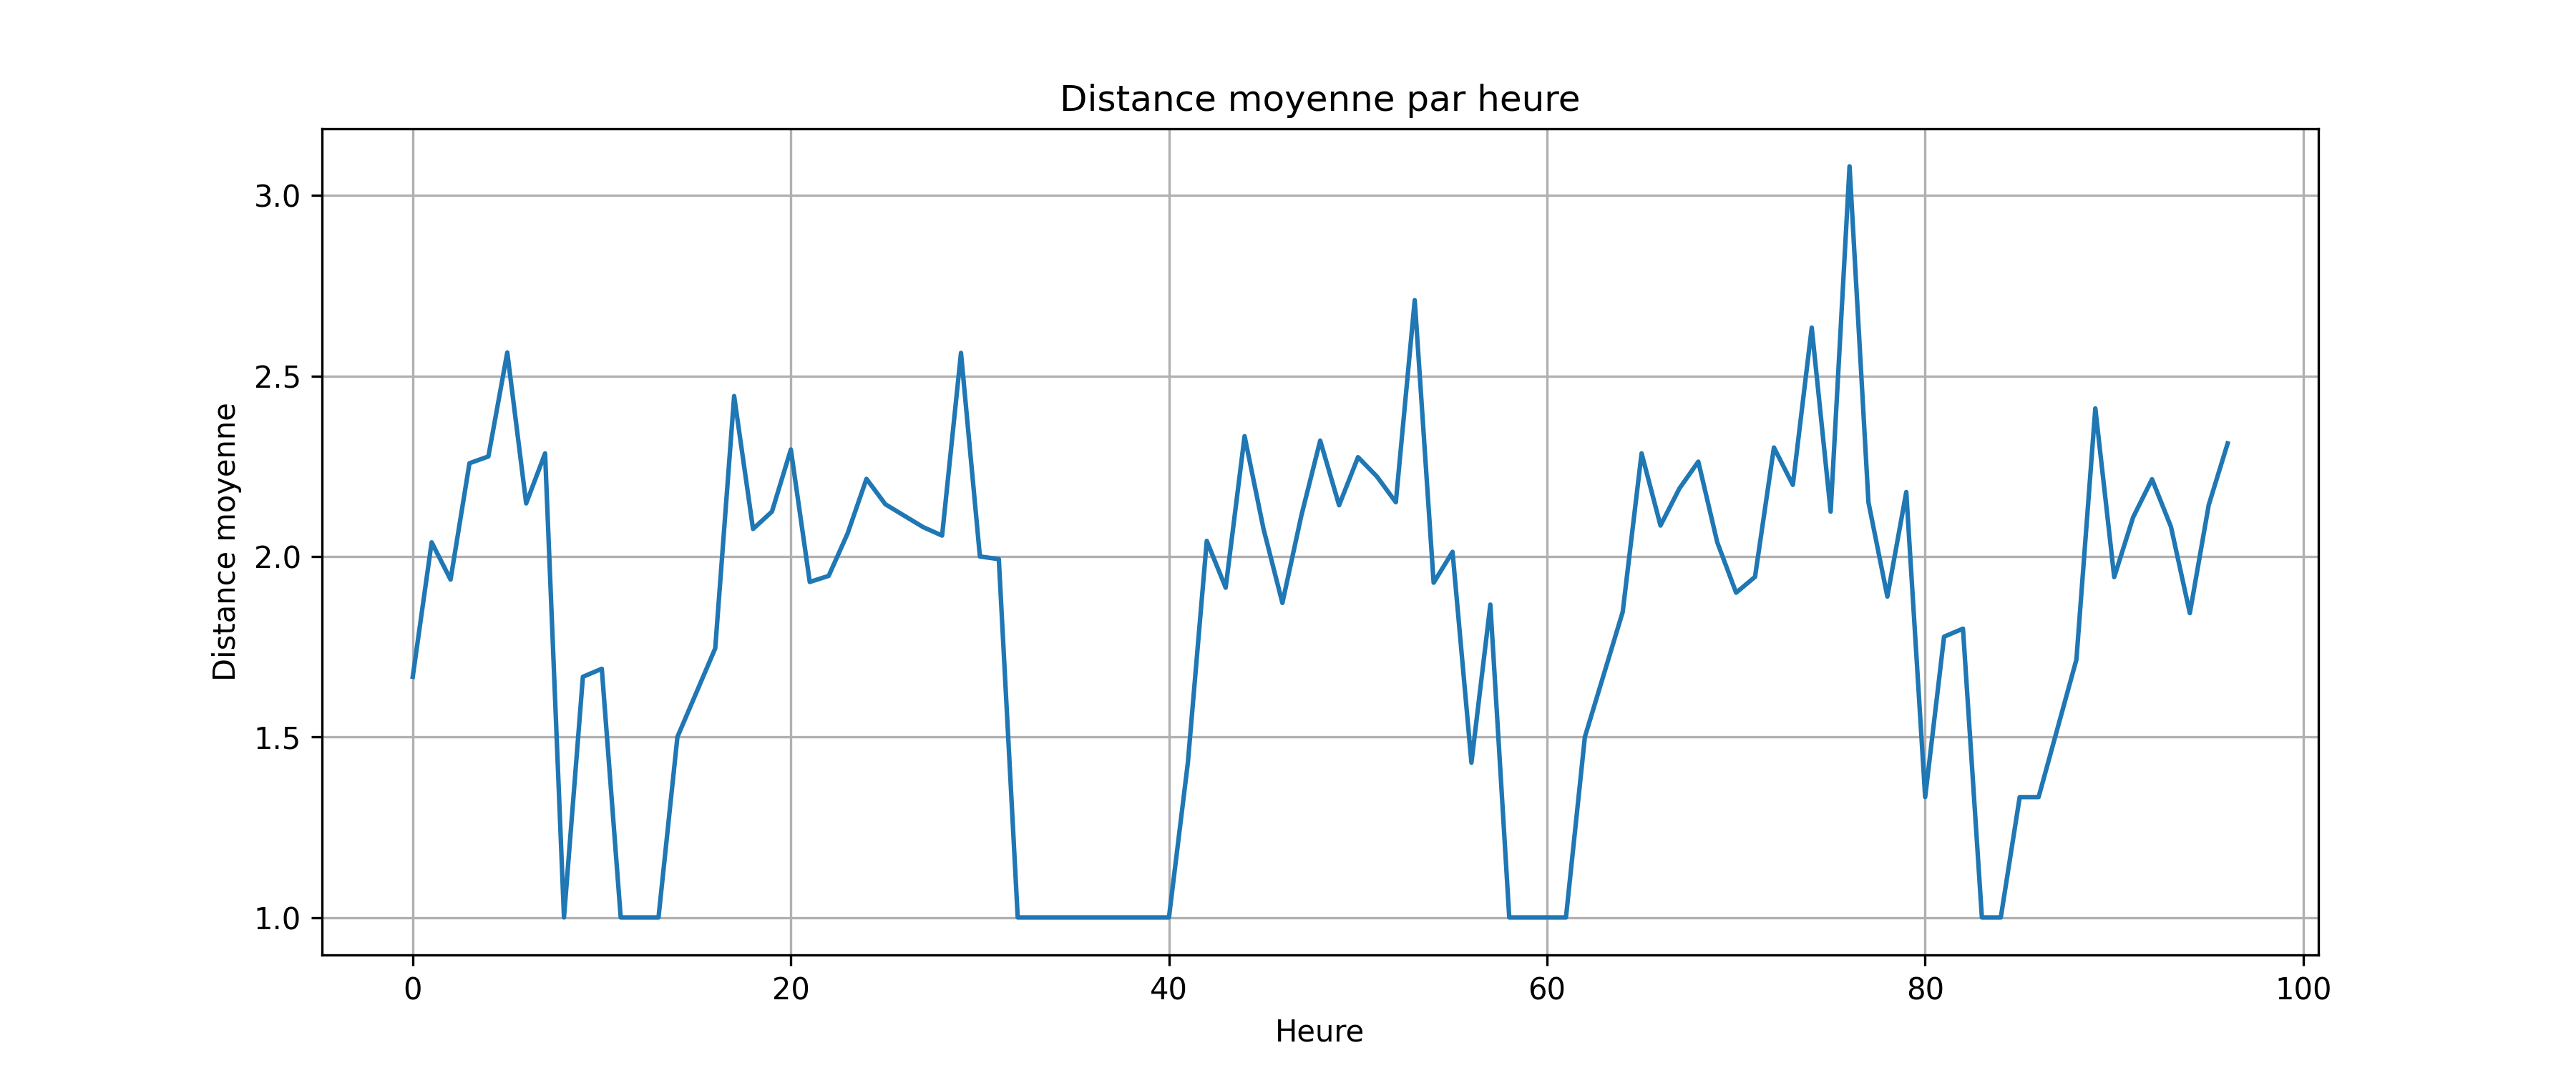
\includegraphics[width=0.90\linewidth]{images/article1/Figure_E3_distance_moyenne.png}
\caption{Distance moyenne par heure.}
\end{figure}

Avec une distance moyenne entre 1.8 et 2.6, l’information (ou un agent infectieux) peut se propager très rapidement.

\subsection{Nombre de composantes}

\begin{figure}[H]
\centering
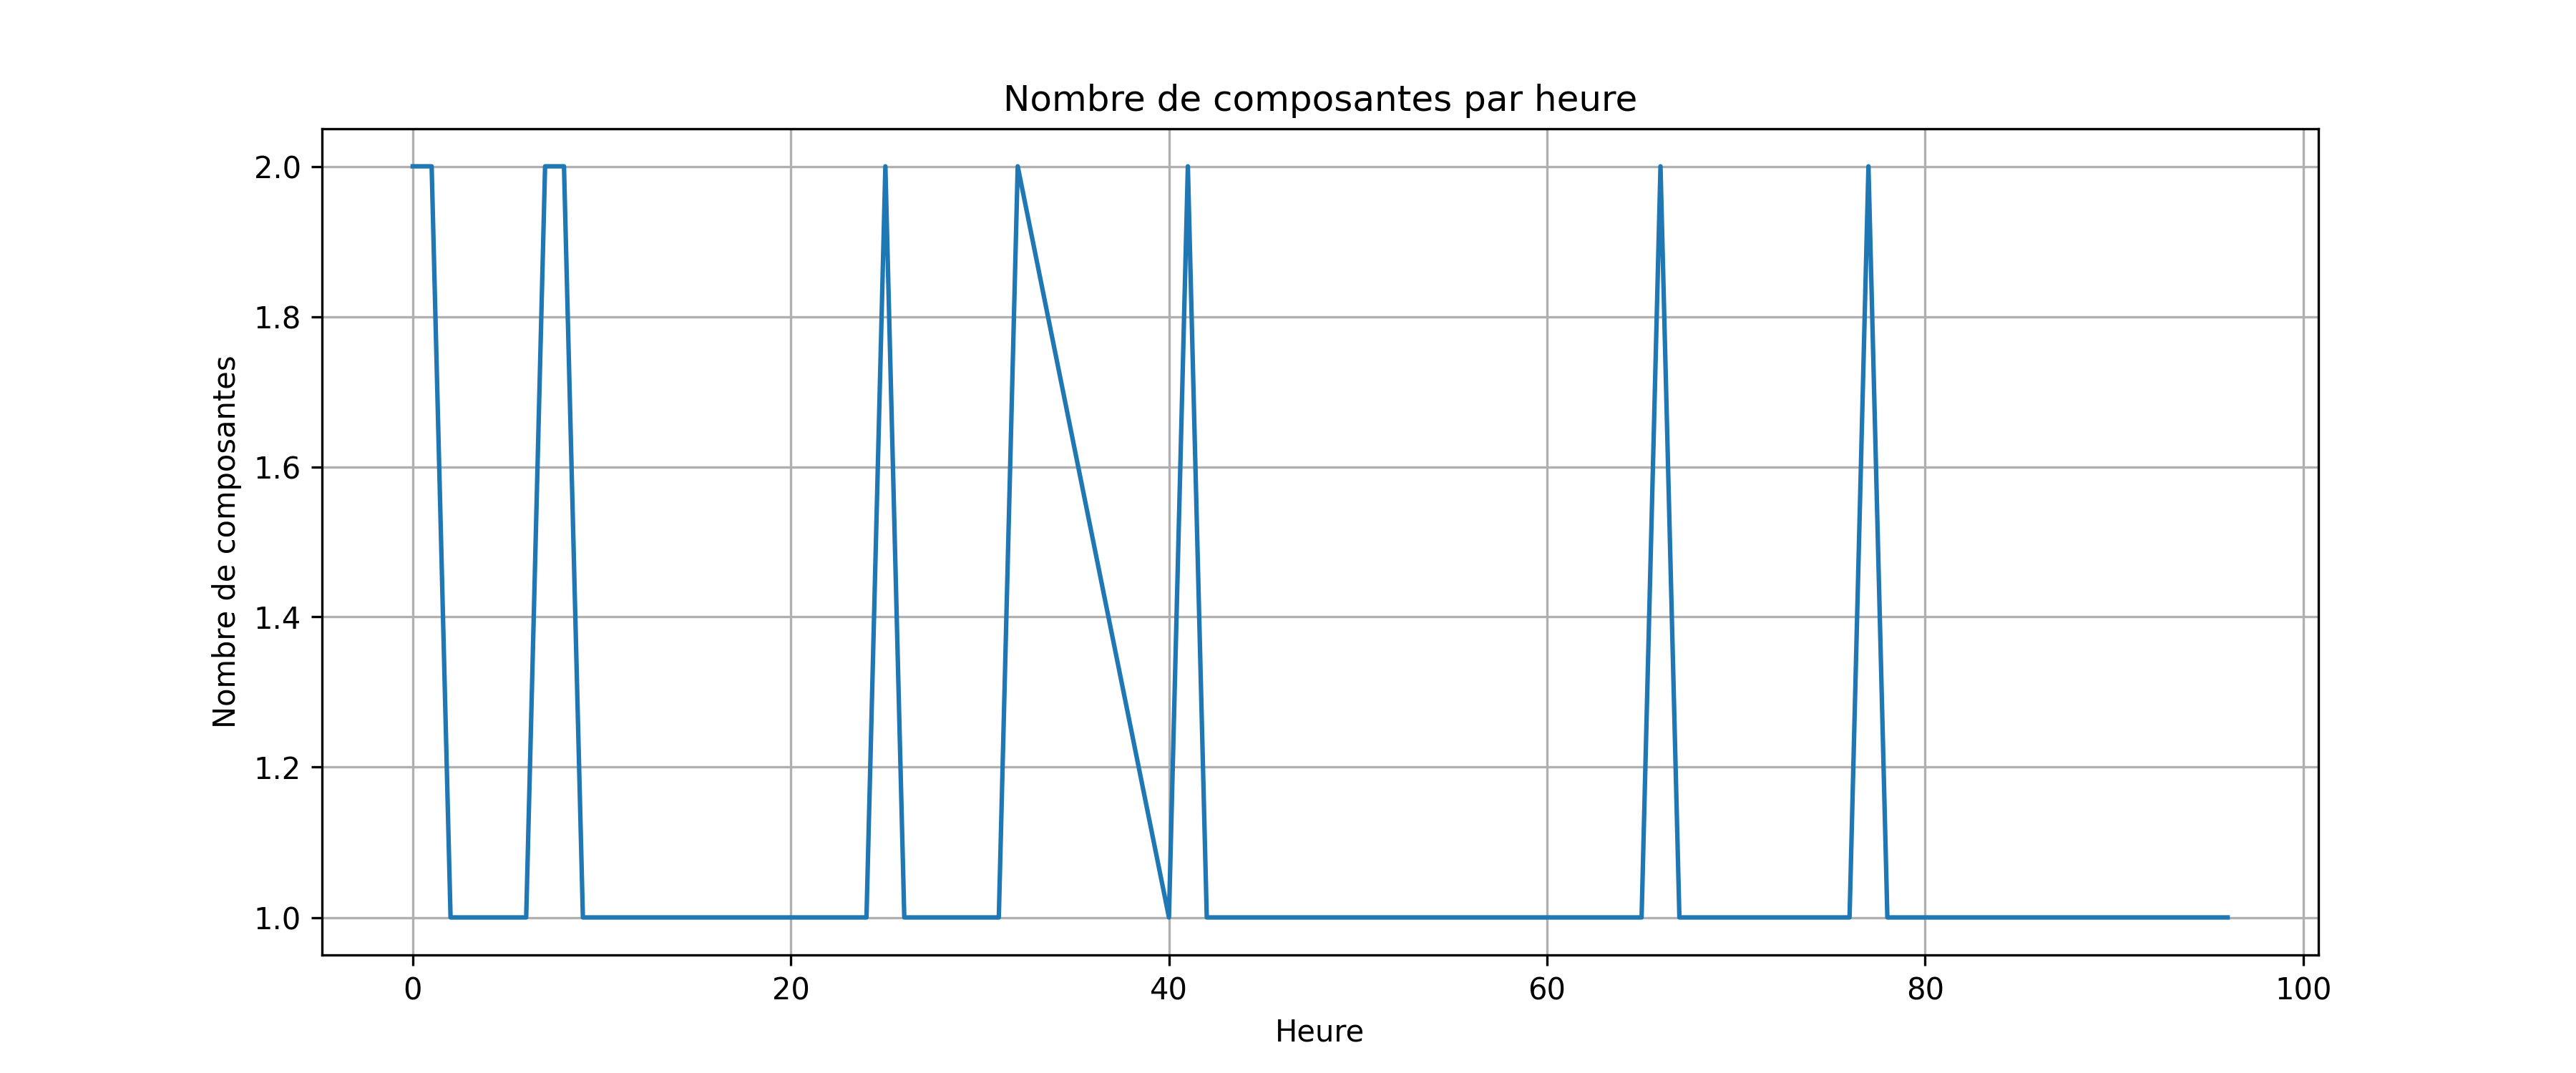
\includegraphics[width=0.90\linewidth]{images/article1/Figure_E4_composantes.png}
\caption{Nombre de composantes du graphe.}
\end{figure}

Le réseau reste quasi toujours connecté : forte cohésion structurelle, faible fragmentation.

% ============================================================
\section{Graphe agrégé : visualisation et communautés}
% ============================================================

Le graphe agrégé résume l’ensemble des contacts sur la période :
\textbf{75 nœuds} et \textbf{1139 arêtes}, donc un réseau très dense.

\subsection{Visualisation brute}

\begin{figure}[H]
\centering
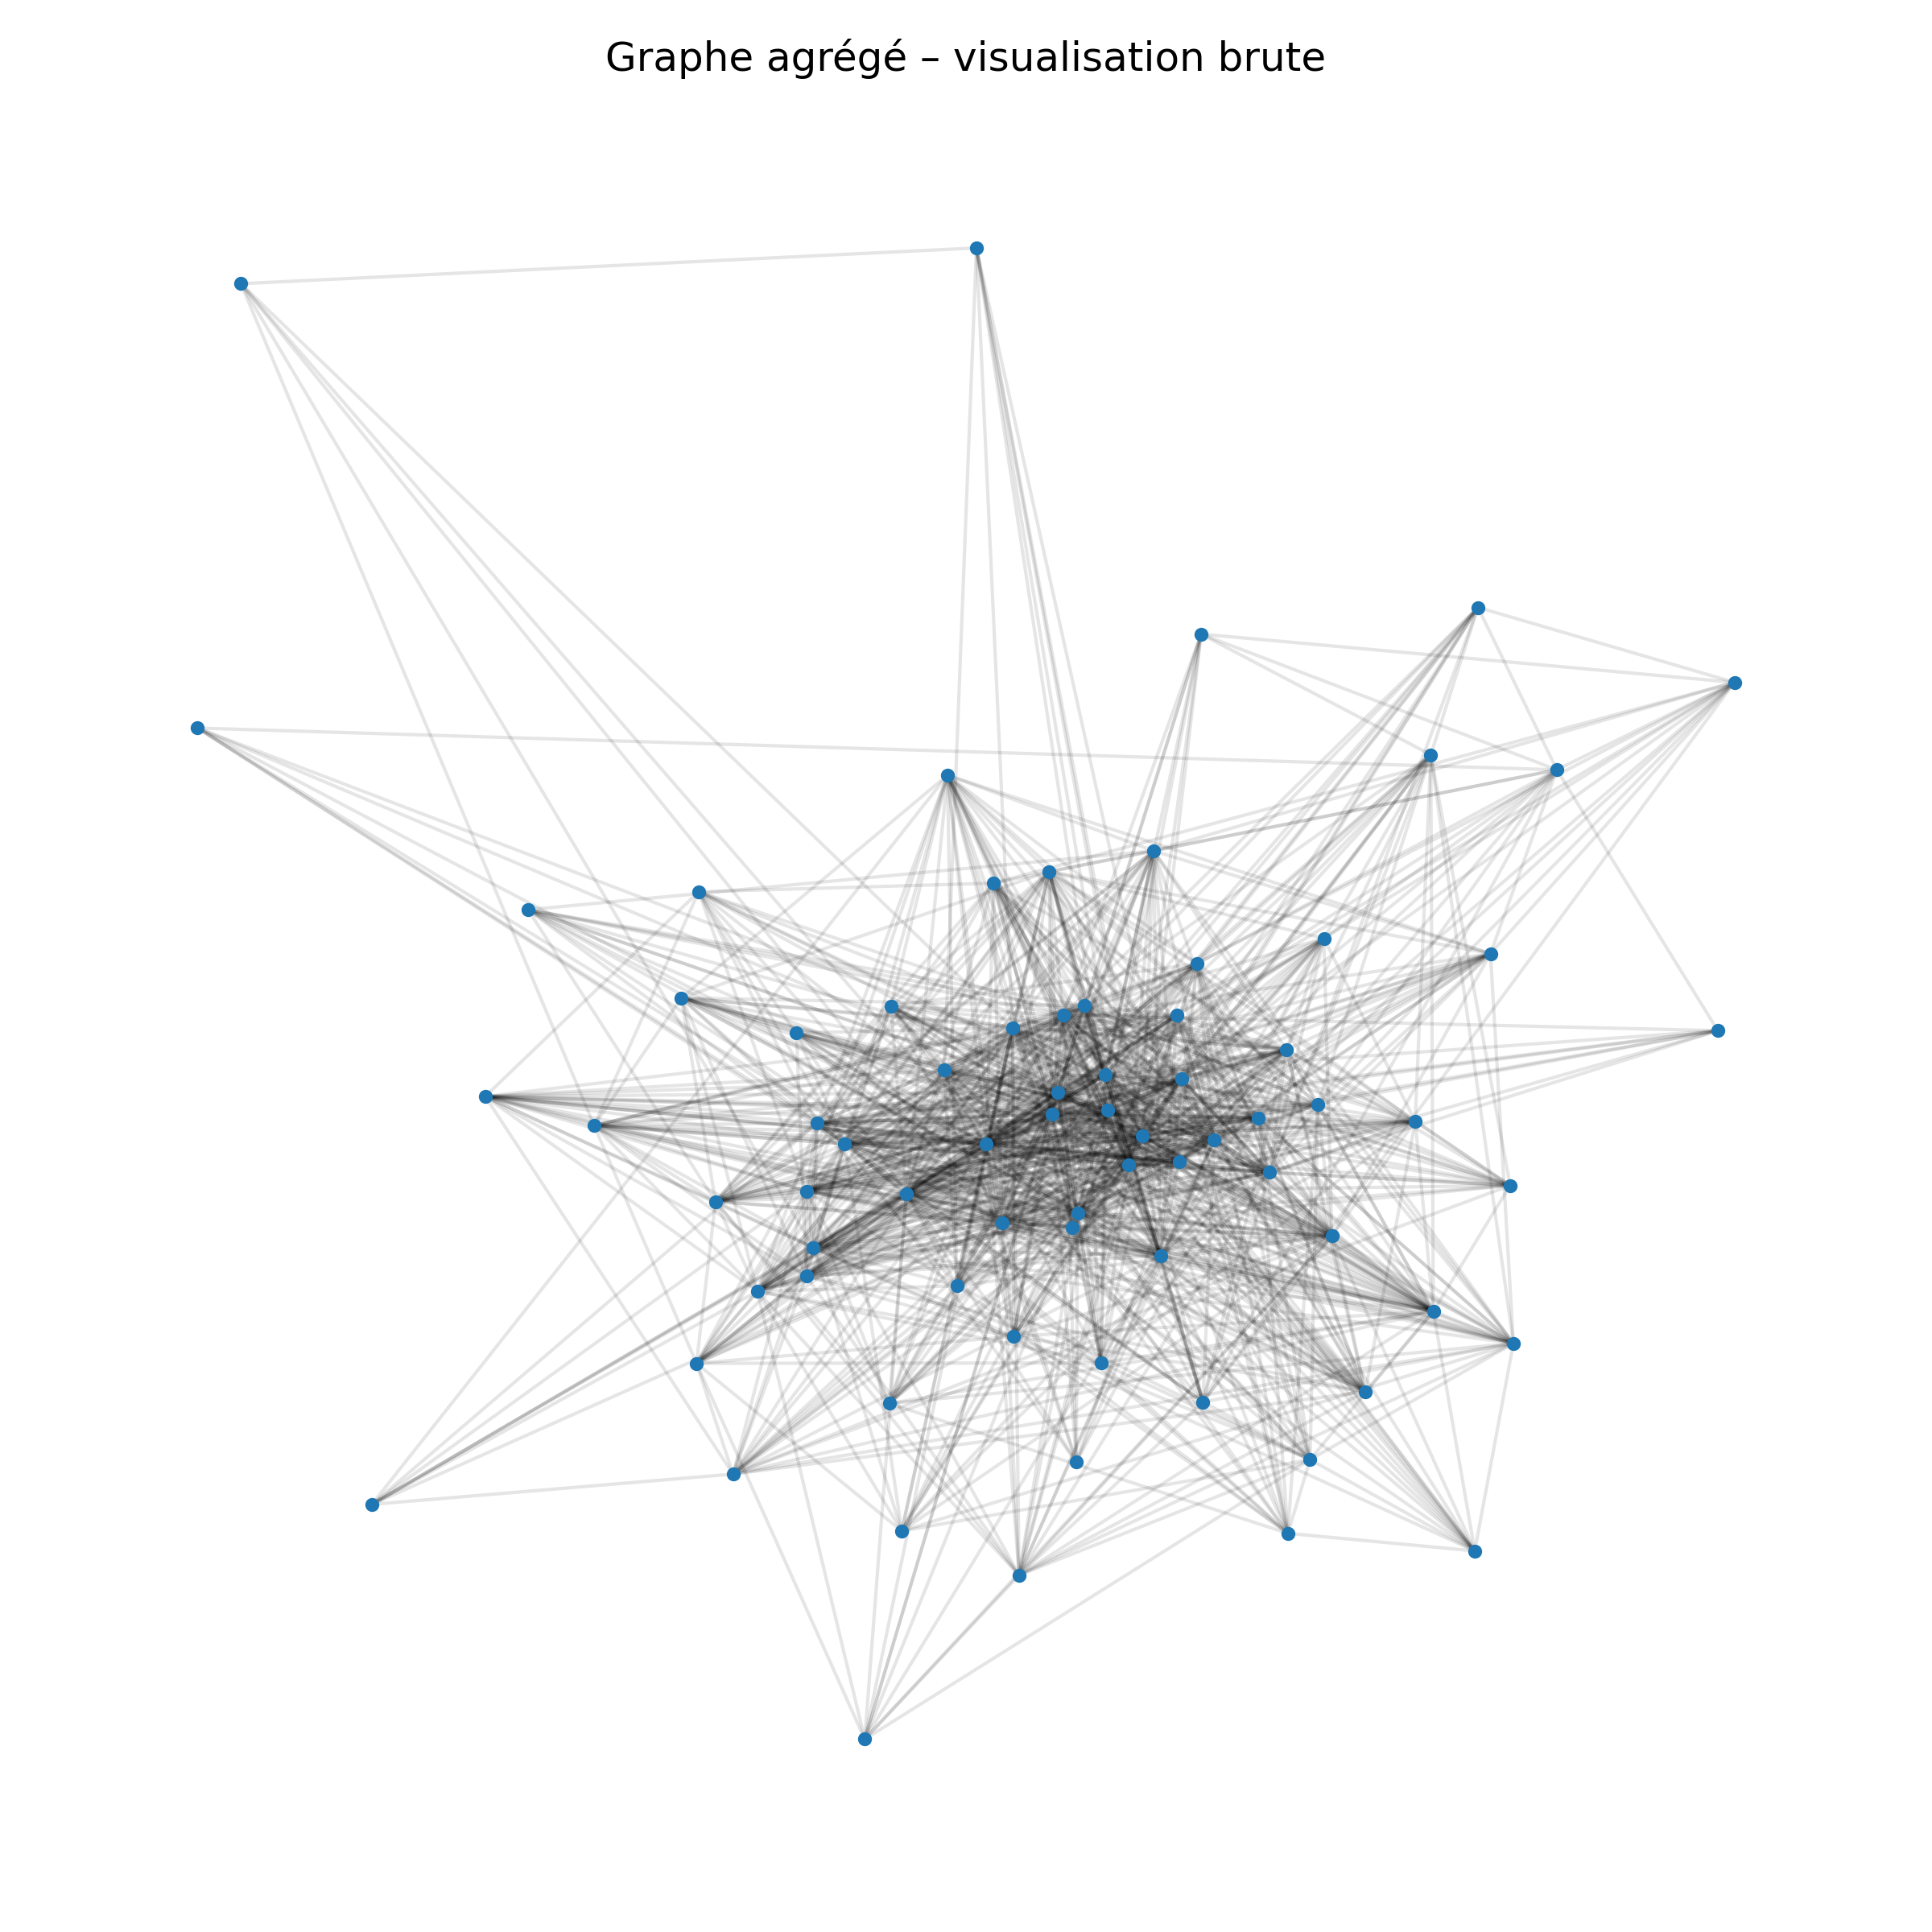
\includegraphics[width=0.75\linewidth]{images/article1/Figure_D0_graphe_brut.png}
\caption{Graphe agrégé : visualisation brute.}
\end{figure}

La densité élevée rend la zone centrale très saturée, typique d’un noyau de personnel fortement interconnecté.

\subsection{Détection de communautés (Louvain)}



\begin{figure}[H]
\centering
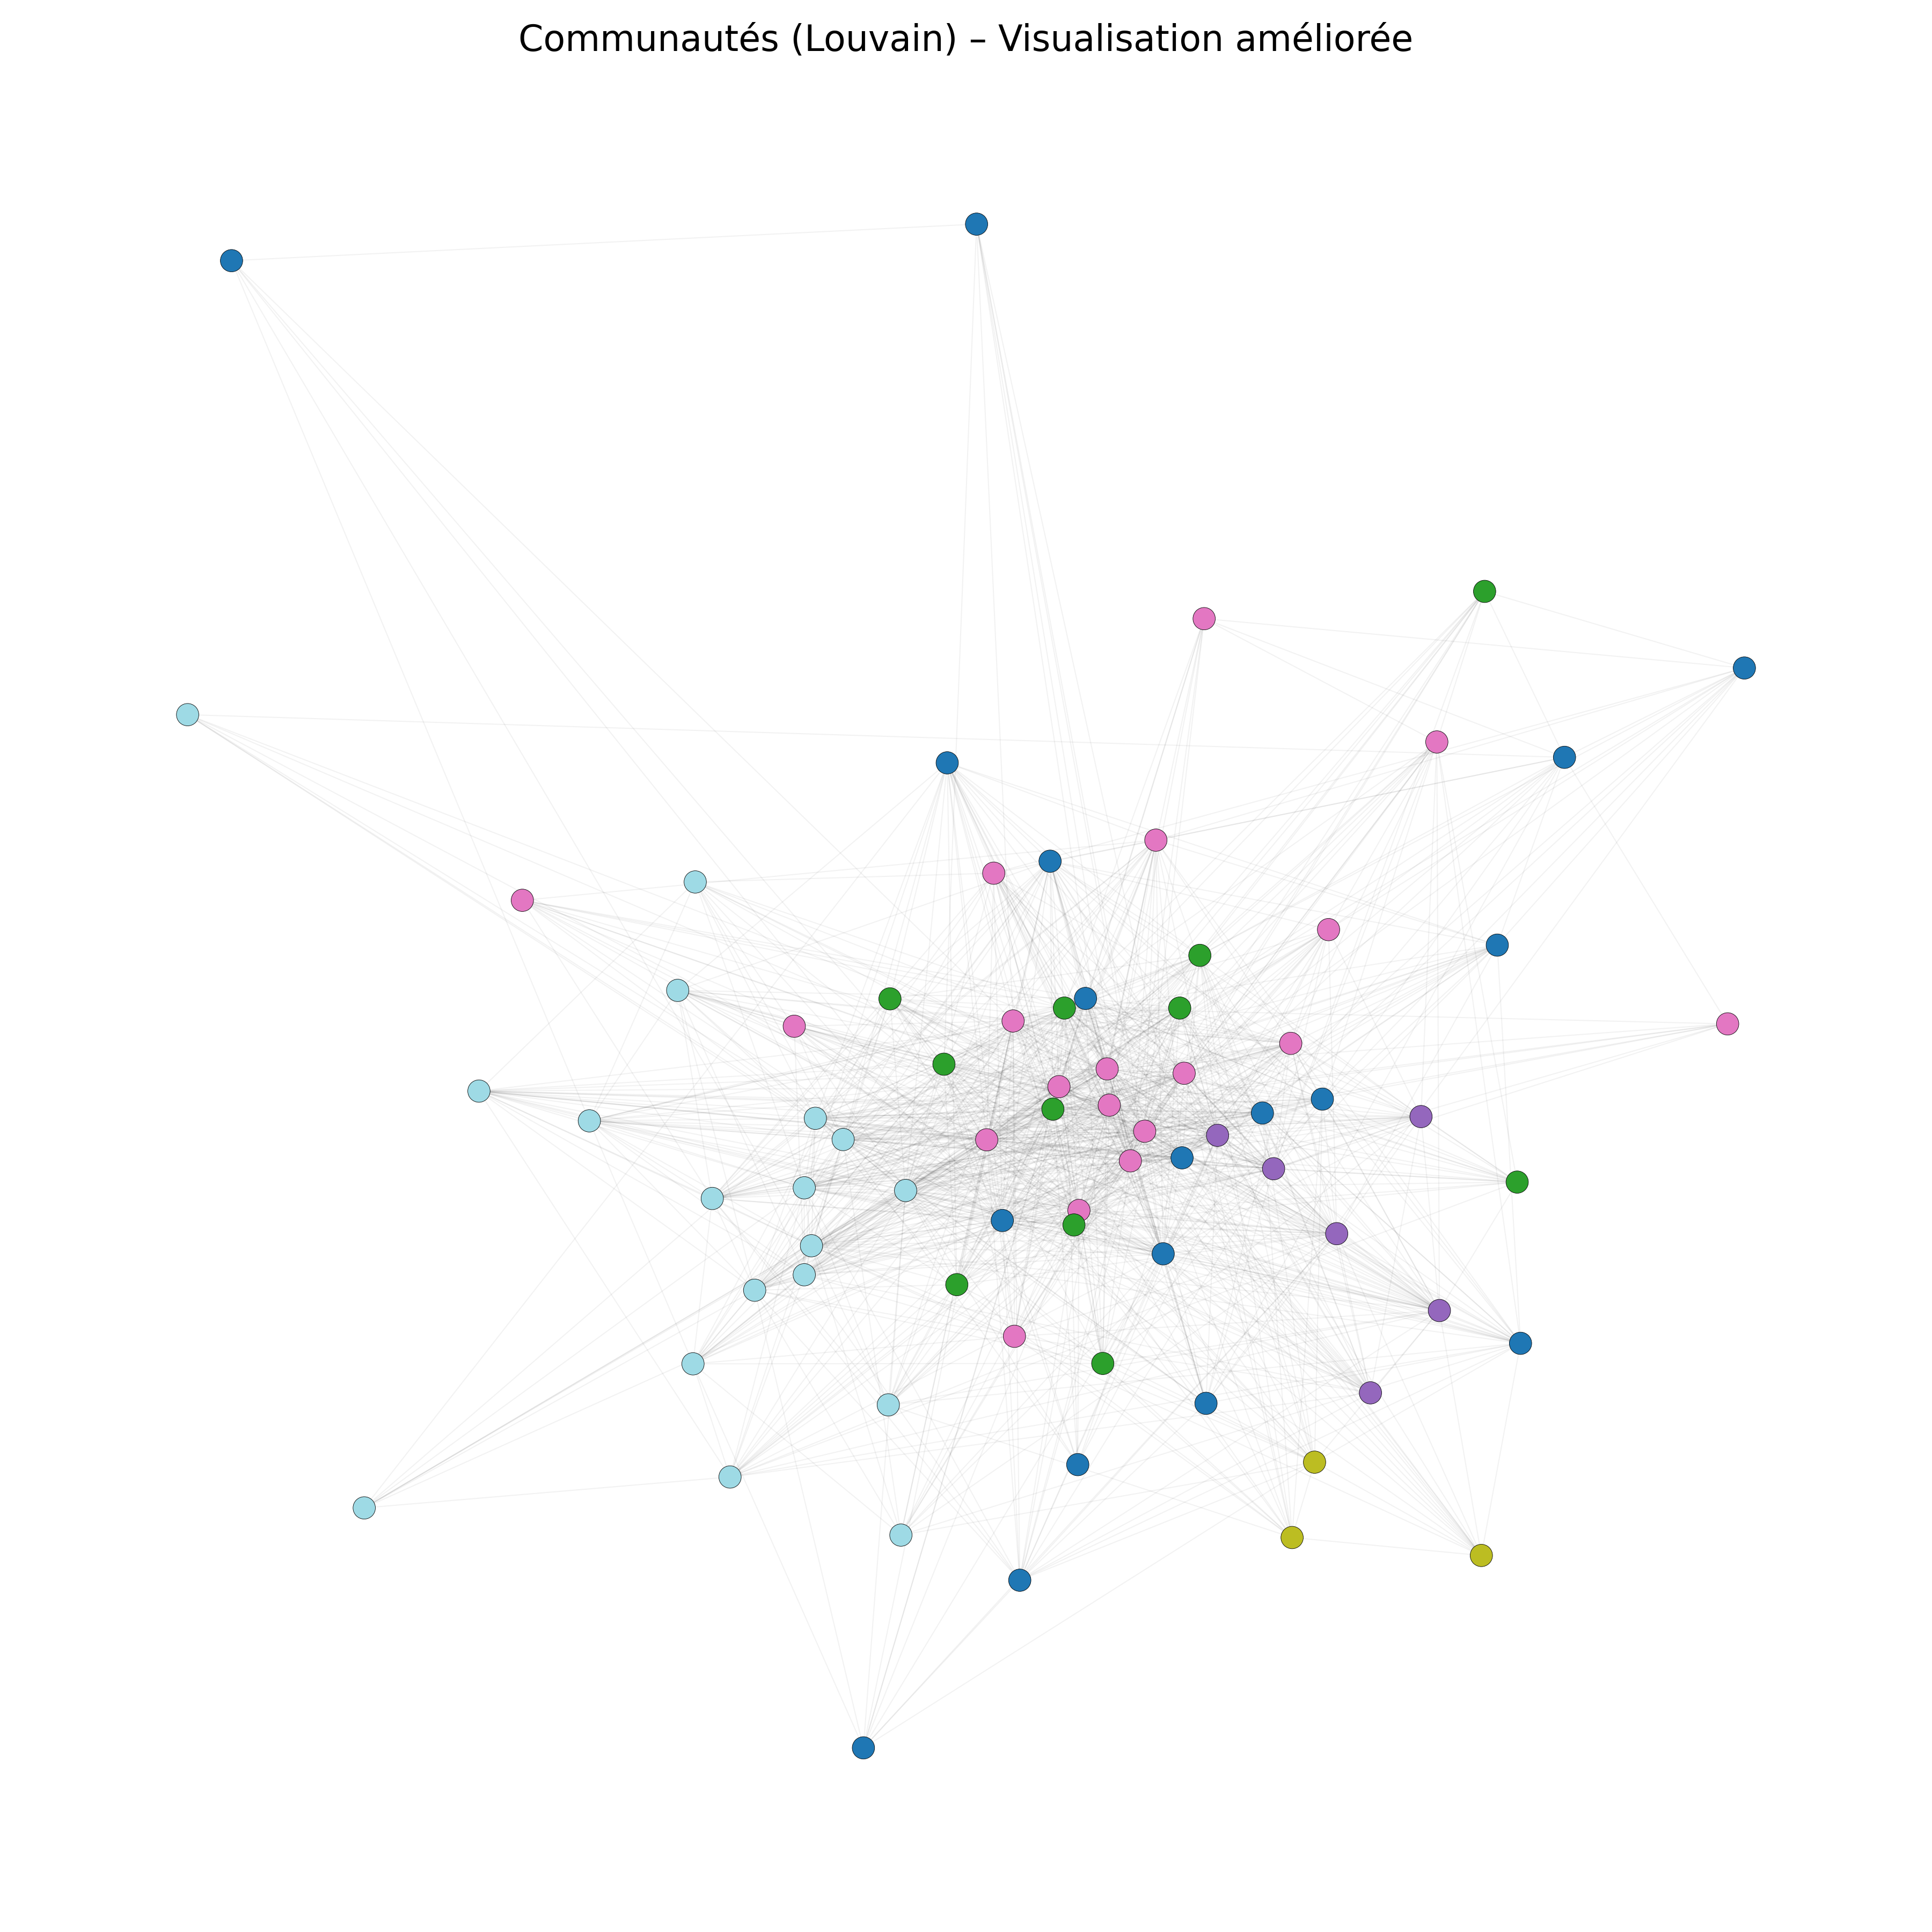
\includegraphics[width=0.75\linewidth]{images/article1/Figure_D1_communautes_améliorée.png}
\caption{Communautés détectées.}
\end{figure}

Le réseau présente \textbf{6 communautés} avec une modularité de \textbf{0.368}, indiquant une structure communautaire \textbf{modérée}.  
Ces modules correspondent plausiblement à des équipes soignantes, ou à des sous-ensembles “patients + personnel référent”.

% ============================================================
\section{Structure core--périphérie}
% ============================================================

La structure core--périphérie est identifiée à partir de la probabilité de persistance
$\alpha_S$ sur le graphe agrégé, pondéré par la fréquence des contacts.
La coupure obtenue isole une \textbf{périphérie de 74 nœuds} et un \textbf{core réduit à un seul individu}
(ID \textbf{1115}, rôle \textbf{NUR}).

La courbe $\alpha_S$ reste nulle sur la majorité des étapes, puis augmente brutalement
lorsque ce nœud est inclus, indiquant une forte centralisation des interactions.
La périphérie regroupe l’ensemble des autres rôles (patients, médecins et administratifs),
tandis que le noyau correspond à un infirmier particulièrement dominant,
en cohérence avec les résultats obtenus sur les centralités.

% ============================================================
\section{Interprétation générale}
% ============================================================

Les résultats obtenus confirment une organisation des contacts hospitaliers
fortement structurée et hétérogène.
Les analyses montrent qu’un nombre limité d’infirmiers, et dans une moindre mesure
de médecins, concentre une part importante des interactions, tant en nombre
qu’en durée, et occupe des positions centrales dans la connectivité globale du réseau.
Ces individus correspondent aux profils identifiés dans l’article comme
potentiels super-contacteurs parmi les professionnels de santé.

La comparaison avec des graphes de référence indique que cette organisation
ne peut être expliquée par le hasard ni par la seule distribution des degrés.
La présence d’un clustering élevé et de motifs d’interaction dépendants des rôles
reflète des contraintes fonctionnelles liées au fonctionnement de l’hôpital.

L’étude temporelle met en évidence des cycles journaliers marqués,
avec des pics d’activité en journée et une baisse nette la nuit,
tout en montrant une stabilité globale des patterns de contacts d’un jour à l’autre.
Enfin, l’organisation communautaire et la structure core--périphérie
révèlent un noyau dense principalement composé de soignants,
entouré d’une périphérie dominée par les patients.

Dans l’ensemble, ces observations sont cohérentes avec les conclusions de l’article
et soulignent le rôle central du personnel soignant dans la structuration
et la dynamique des contacts hospitaliers.\\
\\
\\
\\
\\
\\
\\
\\
\\
\\
\\
\\
\\
\\
\\
% ============================================================
\begin{thebibliography}{99}

\bibitem{ozella2021}
L. Ozella, D. Paolotti, G. Lichand, J.-P. Rodríguez, S. Haenni,
J. Phuka, O. B. Leal-Neto, C. Cattuto,
\textit{Using wearable proximity sensors to characterize social contact patterns
in a village of rural Malawi},
EPJ Data Science, 10:46, 2021.

\bibitem{vanhems2013}
P. Vanhems, A. Barrat, C. Cattuto, J.-F. Pinton, N. Khanafer,
C. Régis, B.-A. Kim, B. Comte, N. Voirin,
\textit{Estimating Potential Infection Transmission Routes in Hospital Wards Using
Wearable Proximity Sensors},
PLoS ONE, 8(9): e73970, 2013.
doi:10.1371/journal.pone.0073970.

\bibitem{lambiotte_graphmining}
R. Lambiotte,
\textit{Graph Mining},
Notes de cours, Université de Namur, 2023--2024.

\end{thebibliography}


\end{document}



